Among the available topologies in the literature, the most popular has been investigated in section~\ref{sec:comp-delay-design}: the Strong ARM latch and the Double Tail comparator. With a digital clocking scheme different between the SAR of the last stage and the two first stages of the hybrid ADC, a fast version and a slow version of comparators are targeted. The slow version is well-suited for the SAR for which the offset is the most stringent constraint. While for the two first stages, to wit, the Incremental-\(\Delta \Sigma\) and the Algorithmic, require a comparator to make decisions very fast with less constraints on the offset.

For the slow version of comparators, the expected delay should be lower than 3 ns, while the offset does not exceed 10 mV. The hysteresis and differential kickback should be minimized. For the fast version, the delay should be a few hundreds of picoseconds. And the offset is not a big deal since the two first stage combined can be calibrated to cope with up to 50 mV of offset (amplifier offset plus the comparator offset taking into account the capacitive bench).

In consequence, comparators should be tested with respect to the following criteria from -40\(\degree\)C to +175\(\degree\)C\@:
\begin{itemize}
\item The power consumption
\item The offset
\item The time delay
\item The noise
\end{itemize}

For the comparators test chip, DOE\_COMP, there are three test patterns: one to estimate the delay, one to measure only the offset, and a last to estimate the offset, the noise, and the hysteresis. Respectively we called them test pattern A, B, and C. To this, two other measures are required: the power consumption of comparators and the temperature inside the chip. 

% Depicted in the \figurename~\ref{fig:test-chip-comp-patterns} a and e, the Delay measurement circuit is a frequency generator based on the output of the comparator. To measure the offset, the circuit in the \figurename~\ref{fig:test-chip-comp-patterns} b and f, is a regulation loop of one comparator input with a charge pump. The difference between inputs corresponds to the input referred offset of the comparator. And the conventional offset measurement circuit is counting the occurrence of the comparator output for a given differential input, \figurename~\ref{fig:test-chip-comp-patterns} c. The offset, the hysteresis, and the noise can be then extracted from the cumulative distribution function of the output with respect to the differential input voltage.

DOE\_COMP evaluates two different comparator topologies by the mean of dedicated test circuits. This test chip counts up to 20 comparators with 16 comparators under the test pattern C, 8 of each topology. Other test patterns can only test one comparator. Therefore, DOE\_COMP counts two delay test pattern (Pattern A-SA and Pattern A-DTL) and two Offset Feedback test pattern (Pattern B-SA and Pattern B-DTL) to assess each topology. Due to its novelty, one extra Pattern A circuit is added to the test chip for diagnostic purpose with an external comparator. In consequence, DOE\_COMP characterizes 10 Double-Tail latches and 10 Strong-Arm latches with 3 Patterns A, 2 Patterns B, 1 Pattern C and 4 frequency dividers to output high speed signals generated by Pattern A circuits, and to verify the clock connection. 

\begin{figure}[htp]
    \centering
    \begin{subfigure}[b]{0.5\textwidth}
        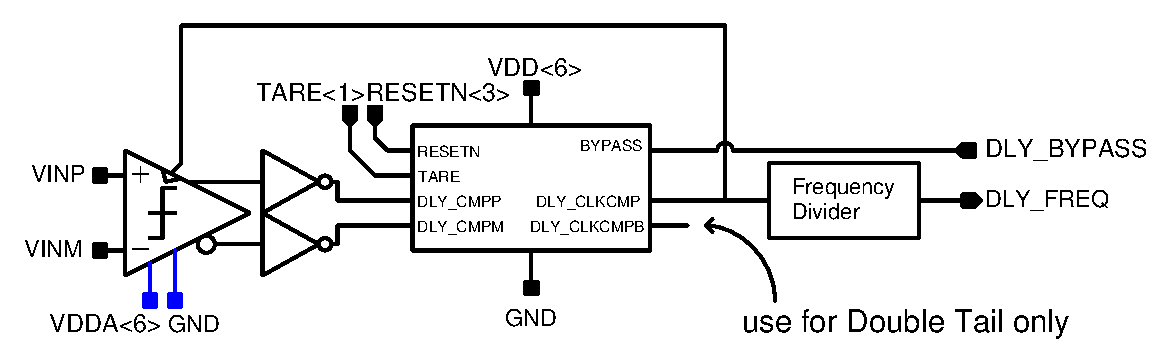
\includegraphics[width=\textwidth]{Chapter5/Figs/comp_test/test_delay_bloc_close_sa.ps}
        \subcaption{Pattern A-SA}
    \end{subfigure}
    \begin{subfigure}[b]{0.5\textwidth}
        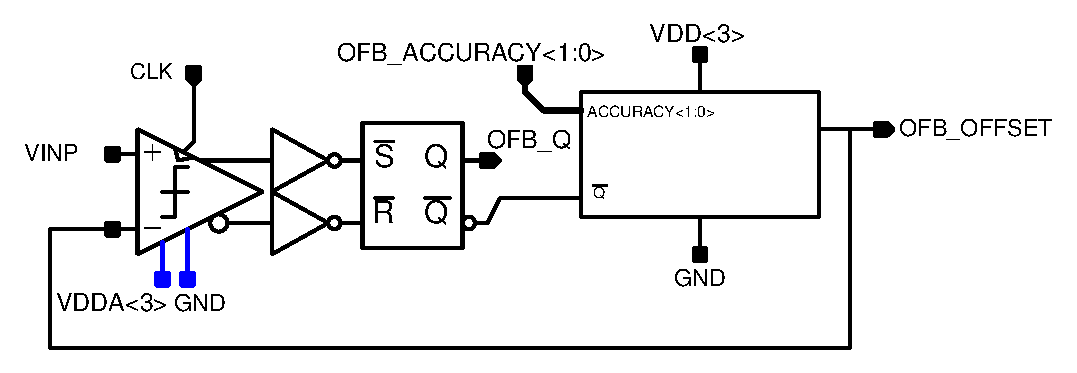
\includegraphics[width=\textwidth]{Chapter5/Figs/comp_test/test_offset_bloc_close_sa.ps}
        \subcaption{Pattern B-SA}
    \end{subfigure}
    \begin{subfigure}[b]{0.75\textwidth}
        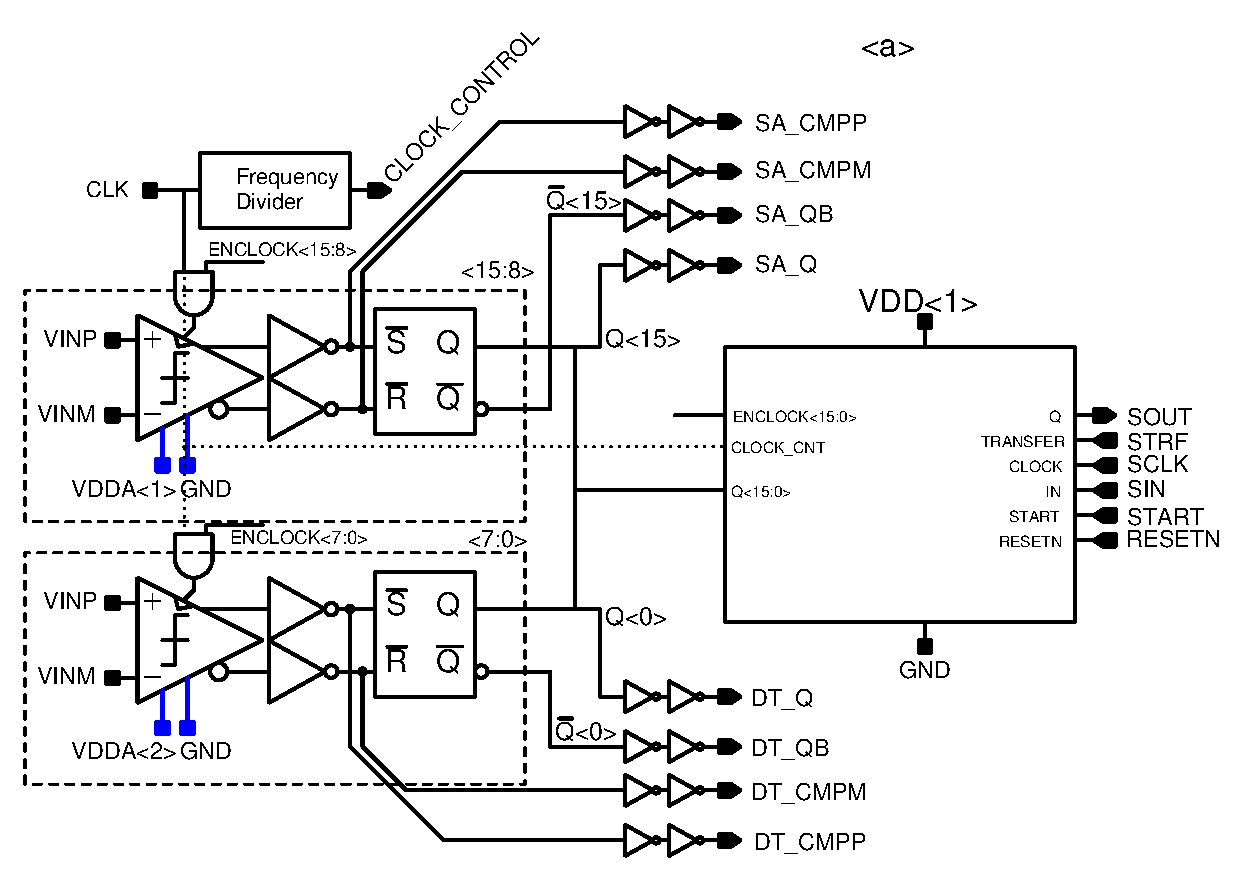
\includegraphics[width=\textwidth]{Chapter5/Figs/comp_test/test_offset_conv_bloc.ps}
        \subcaption{Pattern C}
    \end{subfigure}
    \caption{Representation of test patterns which will be described in the following sections}
    \label{fig:test-chip-comp-patterns}
\end{figure}

Furthermore, one pad will distribute the clock signal CLK across the offset test circuits and their digital part. The signal of the clock is single-ended and will be generated by using a 100 MHz reshaped sine wave.

For signal generation the Tektronic AFG3102C is at our disposal. On the PCB, a clock driver and an impedance adaptation are assumed close to the comparator test chip. Inside the chip, the clock signal reshaped with a Schmitt trigger is distributed differentially across the test chip (CLK and CLKB). A CLOCK\_CONTROL signal is output in order to check to good-connection of the clock signal to test blocks.

The digital signals are generated by an NI-USB 8452 and drive directly pads of the test chip. Inside the IC, those signals are reshaped with a Schmitt trigger. Finally the test chip has 56 pads in total connected to the footprint of a CLCC68 package.

\subsection{Power Consumption}
To supply DOE\_COMP, one power supply is connected to the comparators while another is connected to the remaining circuits.
As both topologies of comparators are tested, we thus separate the power supplies of comparators of different topology to limit the interference in results. As presented in table~\ref{tbl:test-chip-comp-pattern}, there are 12 pads for supply connections: VDDA<6:1> and VDD<6:1>. Therefore, we are able to measure both the comparator power consumption and the test circuit consumption without interference of one over another. For the sake of simplicity, there is one ground pad for all comparators, and one ground for the remaining circuits in DOE\_COMP. These two forms a star connection to have the same reference between comparators and test circuits.

\begin{table}[htp]
    \caption{Test pattern implemented to assess each comparator topology}
    \label{tbl:test-chip-comp-pattern}
    \resizebox{\textwidth}{!}{%
    \begin{tabular}{@{}lclcc@{}}
    \toprule
    \multicolumn{1}{c}{} &  & \multicolumn{1}{c}{} & \multicolumn{2}{c}{Power Supply} \\
    \multicolumn{1}{c}{\multirow{-2}{*}{Test Pattern}} & \multirow{-2}{*}{\begin{tabular}[c]{@{}c@{}}Comparator\\ Topology\end{tabular}} & \multicolumn{1}{c}{\multirow{-2}{*}{Function}} & comparator & test circuit \\ \midrule
    Pattern A & Strong Arm &  & VDDA\textless{}6\textgreater{} & VDD\textless{}6\textgreater{} \\
     & Double-Tail & \multirow{-2}{*}{\begin{tabular}[c]{@{}l@{}}Measure the delay and the time to reset\end{tabular}} & VDDA\textless{}5\textgreater{} & VDD\textless{}5\textgreater{} \\
    Pattern B & Strong Arm &  & VDDA\textless{}3\textgreater{} & VDD\textless{}3\textgreater{} \\
     & Double-Tail & \multirow{-2}{*}{\begin{tabular}[c]{@{}l@{}}Measure the offset by using a feedback loop\end{tabular}} & VDDA\textless{}4\textgreater{} & VDD\textless{}4\textgreater{} \\
    Pattern C & Strong Arm &  & VDDA\textless{}1\textgreater{} &  \\
     & Double-Tail & \multirow{-2}{*}{\begin{tabular}[c]{@{}l@{}}Measure the offset\\ by using the output CDF\footnotemark\\for a given input voltages\end{tabular}} & \multicolumn{1}{l}{  VDDA\textless{}2\textgreater{}} & \multirow{-2}{*}{VDD\textless{}1\textgreater{}} \\
     & & & & \\ \bottomrule
    \end{tabular}%
    }
\end{table}
\footnotetext{cumulative density function}

To measure the power consumption, the power supply connections to DOE\_COMP are cut. In normal operation jumpers connect them. For the consumption measurement, an amp-meter takes the place of a jumper.

To limit the variation on power supply pads from the chip consumption, an external capacitor of at least 1 $\mu$F should be connected to each power supply pads. The power supply should be able to provide 20 mA at 1.8 V for digital pads and a peak internal power consumption of 35 mA. For tests, the power consumption of one comparator is in average 20 $\mu$W at 1.8 V. This implies to be able to measure an average current in the order of 11 $\mu$A. A Keithley-2000 series is appropriate with a possible accuracy in the sub micro-amps range. For measures, while only one comparator is connected in the Pattern A and B, the power supply of the Pattern C is connected to 8 comparators.

\subsection{Test Pattern A: Delay Measurement Circuit}
From an junction temperature of -40\(\degree \)C to +175\(\degree \)C, the experimental measurements of the propagation delay pose an interesting challenge. Earlier works have used simple as well as complex circuits for delay extraction. 

The easiest solution would be to externalize the clock and the outputs of the comparator to extract the delay by a high speed high resolution measurement device. Unfortunately, outputs drivers consumes much chip area, add extra delay, bond-wires inductances would alter the signal and the delay estimation too, and different length of cables between the clock of reference and the output generates unconditional error prone measurement system.

For a simple solution of delay measurement, one can generate a DC voltage proportional to the delay. In the case of a clocked comparator, continuous decisions made are averaged by a low-pass filter to externalize a DC voltage. Difficulties occur as a pulse indicates a ``decision made'' event whose width is sensitive to the parasitics and PVT variations. While the PVT variations can be alleviated by the employ of mathematical expressions for differential output pulses as in~\cite{1706643}, it suffers of mismatch in parasitics seen by XOR cells within the pulse of reference generator and the generator of the ``decision made'' pulse.

For instance, high precision time interval measurement systems are commonly used in Telecommunications, nuclear science, frequency synthesis, measurement devices such as oscilloscopes and logic analysers, and time-of-flight cameras are heavily relying on time-to-digital converters (TDC). In a nutshell, a TDC is made with a counter and delay line interpolation~\cite{1637593}. Such converters have a limited achievable accuracy in a technology based on the small delay cell (an inverter), the quantization noise, and the non-linearity in the time interpolation. The latter coming from variation in the delay elements of the smallest delay cell, as the cascade of delay cells increase, the integral non-linearity grows such that accurate measurement of large delay is challenging.

In contrast, measurement circuits based on Vernier delay line can achieve fine delay resolution.

% figure of practical implementations
\begin{figure}[htp]
    \centering
    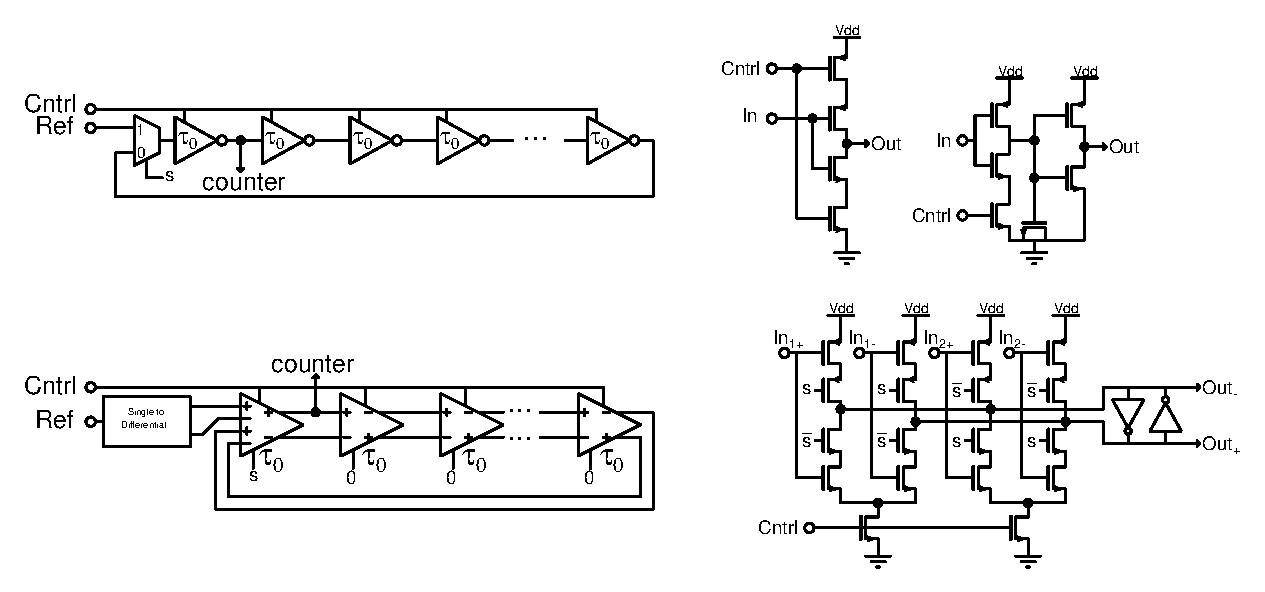
\includegraphics[width=\textwidth]{Chapter5/Figs/delay_line_implementation_possible.ps}
    \caption{Some delay line implementation for the delay estimation and practical implementations of delay cells}
    \label{fig:delay_vernier_interpolation}
\end{figure}

Practical implementations of the delay line and interpolation is depicted by \figurename~\ref{fig:delay_vernier_interpolation}. J.P. Jansson \textit{et al.} use the differential implementation represented in this figure. To estimate the delay a synchronous counter performs a coarse estimation of the delay while the recorded state of the delay line divides the clock of the counter into pieces of \(\Delta T\)~\cite{1637593}. The recorded state of the delay line corresponds to the value stored by DFFs of the positive output of these delay cells.

That said, averaging results either in the time domain or by several TDC running in parallel mitigates the non-linearity: the improvements being inversely proportional to the square root of measurements. However, they are sensitive to PVT variations~\cite{6233014, 5256168} such that calibration is mandatory. Finally, this method does not timely occupy a silicon footprint for built-in self-test.

Finally, the ring oscillator can also be employed to estimate the delay as in~\cite{8267856} wherein perused different oscillators related to the device under test can accurately calculate the delay of element under test. In the case of~\cite{8267856} the delay of Through-Silicon Via for 3D IC are measured. This solution fit within a small silicon area with a large measurement range. Unfortunately, as the number of oscillators increase, mismatch of their instance is averaged and the calculus of the delay becomes even more tedious. Furthermore, it is difficult from the design phase to estimate the accuracy of measurement.
\nomenclature[z]{IC}{Integrated Circuit}

\subsubsection{Principle}
Therefore, we proposed a circuit to reliably measure the comparator's delay with a differential measure of frequency generated by an auto-oscillator with an estimation of the measurement accuracy early in its design phase. The generated frequency is then divided by an arbitrary ratio N to be measured to prevent high speed signal routing consideration.

The auto-oscillator generates a first frequency of reference without the comparator only based on digital cells. Then, with the same digital cells configuration the frequency is generated by fully restored comparator outputs in response to the comparators input voltages when the frequency trigger the comparator.

% image of the layout to give the area
\begin{figure}[htp]
    \centering
    \begin{subfigure}[b]{0.47\linewidth}
	    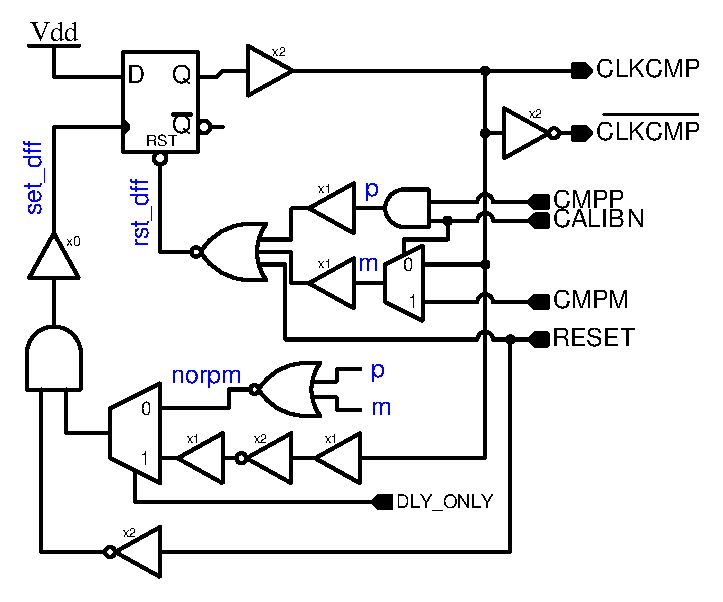
\includegraphics[width=\textwidth]{Chapter5/Figs/test_delay_comp_new_simp.ps}
    \end{subfigure}
    \begin{subfigure}[b]{0.50\linewidth}
	    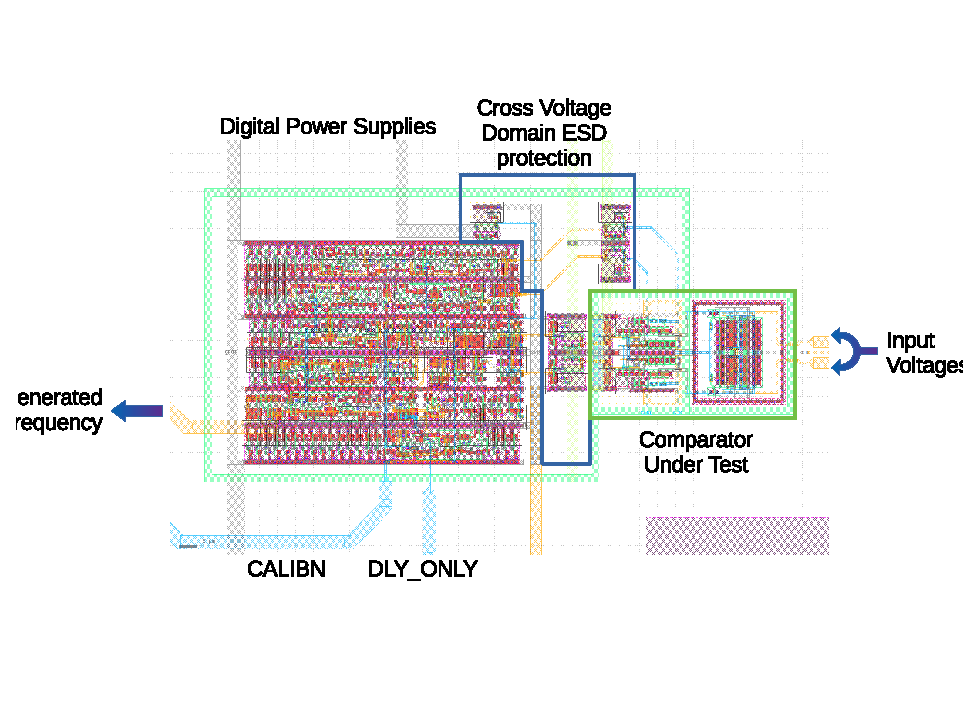
\includegraphics[width=\textwidth]{Chapter5/Figs/layout_delay_meas.eps}
    \end{subfigure}
    \caption{Schematic of the proposed measurement circuit and the delay test dimension}
	\label{fig:meas_circ_schem}
\end{figure}

\figurename~\ref{fig:meas_circ_schem} represents the auto-oscillator circuit connected to the comparator under test. Build around a central D-Flip-Flop generating our frequency CLKCMP, an inverter is used to generate the complementary clock with some delay (\(\approx\)70 ps) to test the Double-Tail comparator.

CALIBN signal allows us to choose the generated frequency: the frequency of reference or the frequency with the comparator to extract the delay. As the comparator required some time to reset, the required time to reset can also be extracted. To select whether we need to extract only the delay or the delay and the reset time of the comparator DLY\_ONLY shall respectively be set to `1' and `0'. And the RESET signal sets the CLKCMP signal to `0' which in turn reset the comparator under test. To change from the generation of one frequency to another, a reset is necessary.

At the moment when the signal RESET is released, the reset signal of the DFF is disengaged and CLKCMP keep its state. Few picoseconds later, the clock signal of the DFF rise to `1'. This edge triggers the DFF which sets its outputs Q to `1', as depicted by the \figurename~\ref{fig:meas_circ_trans} a and b. In consequence, the comparator makes a decision. The DFF is triggered either by the nor of p and m signal if CALIBN is `1' or by the inversion of CLKCMP if CALIBN is `0'. The DFF is reset, and the oscillations begin.

For DLY\_ONLY set to `1', the clock of the DFF (set\_dff) is a delayed \(\overline{CLKCMP}\). Therefore, the time of CLKCMP spend at zero is fixed and PVT dependant. While, for a DLY\_ONLY signal set to `0', the signal set\_dff depends from the generated pulse of the nor gate. In that case, the time that CLKCMP spent at zero is defined by the speed of the comparator to reset.

The frequency difference between the two modes defined by CALIBN corresponds to the mismatch of the MUX inputs selecting either CMPM or CLKCMP, and the delay of the comparator to make a decision. While, the difference introduced by the two states of DLY\_ONLY corresponds to the difference of the delay and the time to reset the comparator. Thus, the proposed circuit is able to extract the delay of the comparator or the delay and the time to reset the comparator.

\begin{figure}[htp]
	\begin{minipage}[b]{0.47\linewidth}
	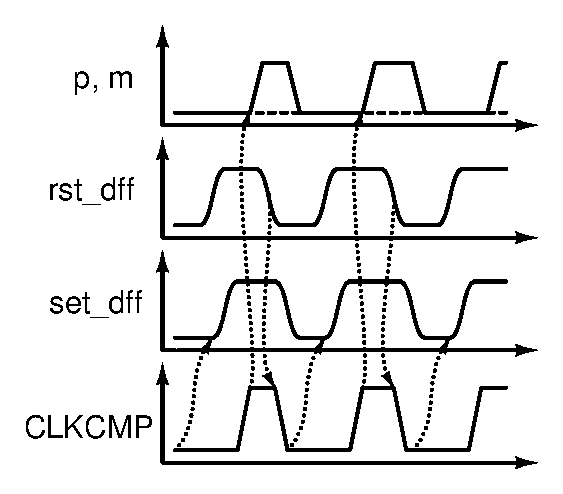
\includegraphics[width=\linewidth]{Chapter5/Figs/test_delay_comp_new_tare0_bypass1.ps}
	\subcaption{CALIBN='0'}
	\end{minipage}
	\begin{minipage}[b]{0.47\linewidth}
	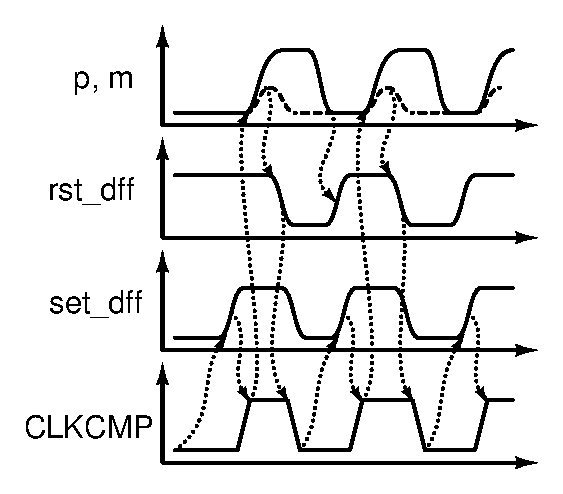
\includegraphics[width=\linewidth]{Chapter5/Figs/test_delay_comp_new_tare1_bypass1.ps}
	\subcaption{CALIBN='1'}
	\end{minipage}
	\caption{Measurement circuit transient behaviour}
	\label{fig:meas_circ_trans}
	\vspace{-1em}
\end{figure}

As the same path is used for the generation of the frequency of reference and the frequency with the comparator under test, the PVT dependence of digital cells is the same in either generation case. Therefore, the differential measurement of the frequency cancels the PVT variations.

The calculation of the frequency in the normal operation mode (CALIBN='1' and DLY\_ONLY=RESET='0') is given by the equation (\ref{eqn:freq_meas_circuit_delay}).

\begin{equation} \label{eqn:freq_meas_circuit_delay}
F_{CLKCMP} = \frac{1}{N} {\left(T_{delay}+T_{set}+T_{rst}+T_{reset}\right)}^{-1}
\end{equation}

where $T_{delay}$ is the delay of the comparator, $T_{reset}$ the time the comparator takes to reset, and $T_{set}$/$T_{rst}$ the time of the digital circuit to react. In detail, $T_{set} = 2 T_{MUX} + T_{NOR} + T_{AND2} + T_{DLY2} + T_{DFF} + T_{BUX2}$ and $T_{rst} = T_{MUX} + T_{DLY} + T_{NOR3} + T_{DFF} + T_{BUX2}$.

In the calibration mode (CALIBN='0' and DLY\_ONLY=RESET='0') the frequency is given by equation (\ref{eqn:freq_calib}).

\begin{equation} \label{eqn:freq_calib}
F_{CLKCMP*} = \frac{1}{N} \left(T_{set}+T_{rst}\right)^{-1}
\end{equation}

The sum of the delay and the reset time is thus given by the equation (\ref{eqn:dly_reset_from_freq}).

\begin{equation}
\label{eqn:dly_reset_from_freq}
T_{delay}+T_{reset} = \frac{1}{N} \left( \frac{1}{F_{CLKCMP}} - \frac{1}{F_{CLKCMP*}} \right)
\end{equation}

When the DLY\_ONLY signal is set to `1', the reset time of the comparator no longer matter, and $T_{reset}$ of the equation (\ref{eqn:freq_meas_circuit_delay}) and (\ref{eqn:dly_reset_from_freq}) is 0.

\subsubsection{Design Criteria}
In this design, both set\_dff and rst\_dff are driven by the same signals: $p$ and $m$. To ensure the stability of the circuit the race condition to respect is defined by the equation (\ref{eqn:stability_dly_only_0}) if DLY\_ONLY=`0' 

\begin{equation}
\label{eqn:stability_dly_only_0}
T_{DLY} + T_{NOR3} + T_{margin}<& T_{NOR2} + T_{MUX2} + T_{AND2} + T_{DLY2}
\end{equation}

and by equation (\ref{eqn:stability_dly_only_1}) if DLY\_ONLY=`1'.

\begin{equation}
\label{eqn:stability_dly_only_1}
T_{MUX} + T_{DLY} & + T_{NOR3} + T_{margin} < T_{INV} + 2T_{DLY} + T_{MUX2} + T_{AND2} + T_{DLY2}
\end{equation}
And this over the process and temperature variation which limit the measurement delay range of the circuit.

\subsubsection{Measures}
The basic setup for the test in this section is depicted by the \figurename~\ref{fig:doe003_measurebench}. This includes four power supplies, a frequency meter, a multimeter, an optional oscilloscope, and an optional current source.

Among power supplies, two are for the power distribution. One a 1.8 V for the core and one at 3.3 V for the level shifting needed of the digital signals connected to NI-USB boxes. The remaining two are dedicated to the input voltages applied at comparator's inputs.

The frequency meter should be plugged in the BNC signal of at the top of the motherboard named SA\_DLY\_FREQ1 and DT\_DLY\_FREQ1.

\begin{figure}[htp]
    \centering
    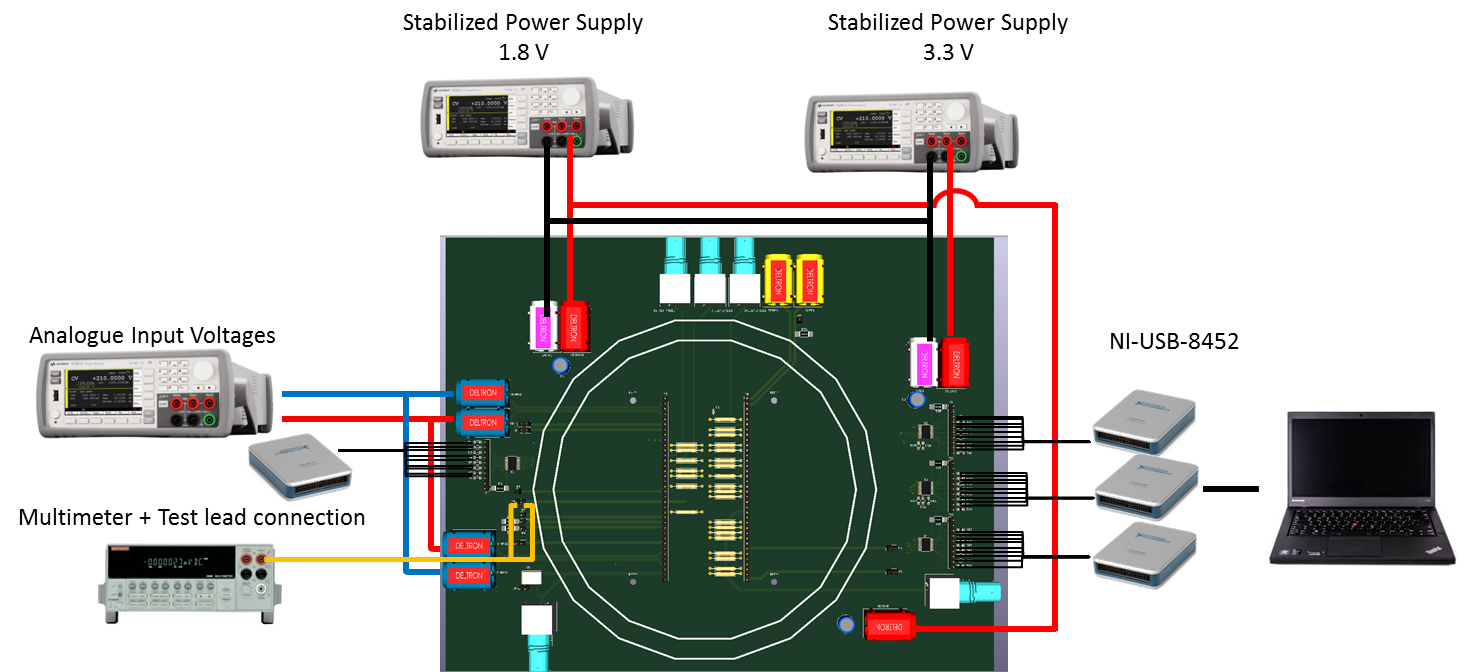
\includegraphics[width=.8\textwidth]{Chapter5/Figs/delay_board_setup.png}
    \caption{Bench-Top installation to measure the delay of comparators}
    \label{fig:doe003_measurebench}
\end{figure}

Either a homemade software or LabView is required to drive the NI-USB boxes. In our case, they are driven by the Labview API provided into a C code, allowing us to drive pins of SPI port as DIO.

For all possible configurations of CALIBN and DLY\_ONLY signals, we measure the frequencies generated for the following temperatures: -40$\degree$C, -25$\degree$C, -10$\degree$C, 0$\degree$C, 27$\degree$C, 85$\degree$C, 100$\degree$C, 125$\degree$C, 150$\degree$C, and 175$\degree$C.

Since by design we fixed the frequency divider to be $N = 64$, the delay is given for DLY\_ONLY = `1' by
\begin{equation}
 T_{delay} = \frac{1}{64} \left(\frac{1}{F_{CALIBN=1}}-\frac{1}{F_{CALIBN=0}} \right)
\end{equation}
And the sum of the delay and the time to reset is given for DLY\_ONLY = `0' by
\begin{equation}
    T_{delay}+T_{reset} = \frac{1}{64} \left(\frac{1}{F_{CALIBN=1}}-\frac{1}{F_{CALIBN=0}} \right)
\end{equation}

\begin{figure}[htp]
    \centering
    %% Creator: Matplotlib, PGF backend
%%
%% To include the figure in your LaTeX document, write
%%   \input{<filename>.pgf}
%%
%% Make sure the required packages are loaded in your preamble
%%   \usepackage{pgf}
%%
%% Figures using additional raster images can only be included by \input if
%% they are in the same directory as the main LaTeX file. For loading figures
%% from other directories you can use the `import` package
%%   \usepackage{import}
%% and then include the figures with
%%   \import{<path to file>}{<filename>.pgf}
%%
%% Matplotlib used the following preamble
%%   \usepackage{gensymb}
%%   \usepackage[utf8x]{inputenc}
%%   \usepackage[T1]{fontenc}
%%
\begingroup%
\makeatletter%
\begin{pgfpicture}%
\pgfpathrectangle{\pgfpointorigin}{\pgfqpoint{3.961700in}{2.962412in}}%
\pgfusepath{use as bounding box, clip}%
\begin{pgfscope}%
\pgfsetbuttcap%
\pgfsetmiterjoin%
\definecolor{currentfill}{rgb}{1.000000,1.000000,1.000000}%
\pgfsetfillcolor{currentfill}%
\pgfsetlinewidth{0.000000pt}%
\definecolor{currentstroke}{rgb}{1.000000,1.000000,1.000000}%
\pgfsetstrokecolor{currentstroke}%
\pgfsetdash{}{0pt}%
\pgfpathmoveto{\pgfqpoint{0.000000in}{0.000000in}}%
\pgfpathlineto{\pgfqpoint{3.961700in}{0.000000in}}%
\pgfpathlineto{\pgfqpoint{3.961700in}{2.962412in}}%
\pgfpathlineto{\pgfqpoint{0.000000in}{2.962412in}}%
\pgfpathclose%
\pgfusepath{fill}%
\end{pgfscope}%
\begin{pgfscope}%
\pgfsetbuttcap%
\pgfsetmiterjoin%
\definecolor{currentfill}{rgb}{1.000000,1.000000,1.000000}%
\pgfsetfillcolor{currentfill}%
\pgfsetlinewidth{0.000000pt}%
\definecolor{currentstroke}{rgb}{0.000000,0.000000,0.000000}%
\pgfsetstrokecolor{currentstroke}%
\pgfsetstrokeopacity{0.000000}%
\pgfsetdash{}{0pt}%
\pgfpathmoveto{\pgfqpoint{0.610776in}{0.489099in}}%
\pgfpathlineto{\pgfqpoint{3.757533in}{0.489099in}}%
\pgfpathlineto{\pgfqpoint{3.757533in}{2.814584in}}%
\pgfpathlineto{\pgfqpoint{0.610776in}{2.814584in}}%
\pgfpathclose%
\pgfusepath{fill}%
\end{pgfscope}%
\begin{pgfscope}%
\pgfsetbuttcap%
\pgfsetroundjoin%
\definecolor{currentfill}{rgb}{0.000000,0.000000,0.000000}%
\pgfsetfillcolor{currentfill}%
\pgfsetlinewidth{0.803000pt}%
\definecolor{currentstroke}{rgb}{0.000000,0.000000,0.000000}%
\pgfsetstrokecolor{currentstroke}%
\pgfsetdash{}{0pt}%
\pgfsys@defobject{currentmarker}{\pgfqpoint{0.000000in}{-0.048611in}}{\pgfqpoint{0.000000in}{0.000000in}}{%
\pgfpathmoveto{\pgfqpoint{0.000000in}{0.000000in}}%
\pgfpathlineto{\pgfqpoint{0.000000in}{-0.048611in}}%
\pgfusepath{stroke,fill}%
}%
\begin{pgfscope}%
\pgfsys@transformshift{0.610776in}{0.489099in}%
\pgfsys@useobject{currentmarker}{}%
\end{pgfscope}%
\end{pgfscope}%
\begin{pgfscope}%
\pgftext[x=0.610776in,y=0.391876in,,top]{\fontsize{10.000000}{12.000000}\selectfont \(\displaystyle -40\)}%
\end{pgfscope}%
\begin{pgfscope}%
\pgfsetbuttcap%
\pgfsetroundjoin%
\definecolor{currentfill}{rgb}{0.000000,0.000000,0.000000}%
\pgfsetfillcolor{currentfill}%
\pgfsetlinewidth{0.803000pt}%
\definecolor{currentstroke}{rgb}{0.000000,0.000000,0.000000}%
\pgfsetstrokecolor{currentstroke}%
\pgfsetdash{}{0pt}%
\pgfsys@defobject{currentmarker}{\pgfqpoint{0.000000in}{-0.048611in}}{\pgfqpoint{0.000000in}{0.000000in}}{%
\pgfpathmoveto{\pgfqpoint{0.000000in}{0.000000in}}%
\pgfpathlineto{\pgfqpoint{0.000000in}{-0.048611in}}%
\pgfusepath{stroke,fill}%
}%
\begin{pgfscope}%
\pgfsys@transformshift{1.196219in}{0.489099in}%
\pgfsys@useobject{currentmarker}{}%
\end{pgfscope}%
\end{pgfscope}%
\begin{pgfscope}%
\pgftext[x=1.196219in,y=0.391876in,,top]{\fontsize{10.000000}{12.000000}\selectfont \(\displaystyle 0\)}%
\end{pgfscope}%
\begin{pgfscope}%
\pgfsetbuttcap%
\pgfsetroundjoin%
\definecolor{currentfill}{rgb}{0.000000,0.000000,0.000000}%
\pgfsetfillcolor{currentfill}%
\pgfsetlinewidth{0.803000pt}%
\definecolor{currentstroke}{rgb}{0.000000,0.000000,0.000000}%
\pgfsetstrokecolor{currentstroke}%
\pgfsetdash{}{0pt}%
\pgfsys@defobject{currentmarker}{\pgfqpoint{0.000000in}{-0.048611in}}{\pgfqpoint{0.000000in}{0.000000in}}{%
\pgfpathmoveto{\pgfqpoint{0.000000in}{0.000000in}}%
\pgfpathlineto{\pgfqpoint{0.000000in}{-0.048611in}}%
\pgfusepath{stroke,fill}%
}%
\begin{pgfscope}%
\pgfsys@transformshift{1.591393in}{0.489099in}%
\pgfsys@useobject{currentmarker}{}%
\end{pgfscope}%
\end{pgfscope}%
\begin{pgfscope}%
\pgftext[x=1.591393in,y=0.391876in,,top]{\fontsize{10.000000}{12.000000}\selectfont \(\displaystyle 27\)}%
\end{pgfscope}%
\begin{pgfscope}%
\pgfsetbuttcap%
\pgfsetroundjoin%
\definecolor{currentfill}{rgb}{0.000000,0.000000,0.000000}%
\pgfsetfillcolor{currentfill}%
\pgfsetlinewidth{0.803000pt}%
\definecolor{currentstroke}{rgb}{0.000000,0.000000,0.000000}%
\pgfsetstrokecolor{currentstroke}%
\pgfsetdash{}{0pt}%
\pgfsys@defobject{currentmarker}{\pgfqpoint{0.000000in}{-0.048611in}}{\pgfqpoint{0.000000in}{0.000000in}}{%
\pgfpathmoveto{\pgfqpoint{0.000000in}{0.000000in}}%
\pgfpathlineto{\pgfqpoint{0.000000in}{-0.048611in}}%
\pgfusepath{stroke,fill}%
}%
\begin{pgfscope}%
\pgfsys@transformshift{2.440286in}{0.489099in}%
\pgfsys@useobject{currentmarker}{}%
\end{pgfscope}%
\end{pgfscope}%
\begin{pgfscope}%
\pgftext[x=2.440286in,y=0.391876in,,top]{\fontsize{10.000000}{12.000000}\selectfont \(\displaystyle 85\)}%
\end{pgfscope}%
\begin{pgfscope}%
\pgfsetbuttcap%
\pgfsetroundjoin%
\definecolor{currentfill}{rgb}{0.000000,0.000000,0.000000}%
\pgfsetfillcolor{currentfill}%
\pgfsetlinewidth{0.803000pt}%
\definecolor{currentstroke}{rgb}{0.000000,0.000000,0.000000}%
\pgfsetstrokecolor{currentstroke}%
\pgfsetdash{}{0pt}%
\pgfsys@defobject{currentmarker}{\pgfqpoint{0.000000in}{-0.048611in}}{\pgfqpoint{0.000000in}{0.000000in}}{%
\pgfpathmoveto{\pgfqpoint{0.000000in}{0.000000in}}%
\pgfpathlineto{\pgfqpoint{0.000000in}{-0.048611in}}%
\pgfusepath{stroke,fill}%
}%
\begin{pgfscope}%
\pgfsys@transformshift{3.391631in}{0.489099in}%
\pgfsys@useobject{currentmarker}{}%
\end{pgfscope}%
\end{pgfscope}%
\begin{pgfscope}%
\pgftext[x=3.391631in,y=0.391876in,,top]{\fontsize{10.000000}{12.000000}\selectfont \(\displaystyle 150\)}%
\end{pgfscope}%
\begin{pgfscope}%
\pgfsetbuttcap%
\pgfsetroundjoin%
\definecolor{currentfill}{rgb}{0.000000,0.000000,0.000000}%
\pgfsetfillcolor{currentfill}%
\pgfsetlinewidth{0.803000pt}%
\definecolor{currentstroke}{rgb}{0.000000,0.000000,0.000000}%
\pgfsetstrokecolor{currentstroke}%
\pgfsetdash{}{0pt}%
\pgfsys@defobject{currentmarker}{\pgfqpoint{0.000000in}{-0.048611in}}{\pgfqpoint{0.000000in}{0.000000in}}{%
\pgfpathmoveto{\pgfqpoint{0.000000in}{0.000000in}}%
\pgfpathlineto{\pgfqpoint{0.000000in}{-0.048611in}}%
\pgfusepath{stroke,fill}%
}%
\begin{pgfscope}%
\pgfsys@transformshift{3.757533in}{0.489099in}%
\pgfsys@useobject{currentmarker}{}%
\end{pgfscope}%
\end{pgfscope}%
\begin{pgfscope}%
\pgftext[x=3.757533in,y=0.391876in,,top]{\fontsize{10.000000}{12.000000}\selectfont \(\displaystyle 175\)}%
\end{pgfscope}%
\begin{pgfscope}%
\pgftext[x=2.184154in,y=0.213666in,,top]{\fontsize{8.000000}{9.600000}\selectfont Temperature [\(\displaystyle \degree\)C]}%
\end{pgfscope}%
\begin{pgfscope}%
\pgfsetbuttcap%
\pgfsetroundjoin%
\definecolor{currentfill}{rgb}{0.000000,0.000000,0.000000}%
\pgfsetfillcolor{currentfill}%
\pgfsetlinewidth{0.803000pt}%
\definecolor{currentstroke}{rgb}{0.000000,0.000000,0.000000}%
\pgfsetstrokecolor{currentstroke}%
\pgfsetdash{}{0pt}%
\pgfsys@defobject{currentmarker}{\pgfqpoint{-0.048611in}{0.000000in}}{\pgfqpoint{0.000000in}{0.000000in}}{%
\pgfpathmoveto{\pgfqpoint{0.000000in}{0.000000in}}%
\pgfpathlineto{\pgfqpoint{-0.048611in}{0.000000in}}%
\pgfusepath{stroke,fill}%
}%
\begin{pgfscope}%
\pgfsys@transformshift{0.610776in}{0.489099in}%
\pgfsys@useobject{currentmarker}{}%
\end{pgfscope}%
\end{pgfscope}%
\begin{pgfscope}%
\pgftext[x=0.266640in,y=0.441271in,left,base]{\fontsize{10.000000}{12.000000}\selectfont \(\displaystyle 1.25\)}%
\end{pgfscope}%
\begin{pgfscope}%
\pgfsetbuttcap%
\pgfsetroundjoin%
\definecolor{currentfill}{rgb}{0.000000,0.000000,0.000000}%
\pgfsetfillcolor{currentfill}%
\pgfsetlinewidth{0.803000pt}%
\definecolor{currentstroke}{rgb}{0.000000,0.000000,0.000000}%
\pgfsetstrokecolor{currentstroke}%
\pgfsetdash{}{0pt}%
\pgfsys@defobject{currentmarker}{\pgfqpoint{-0.048611in}{0.000000in}}{\pgfqpoint{0.000000in}{0.000000in}}{%
\pgfpathmoveto{\pgfqpoint{0.000000in}{0.000000in}}%
\pgfpathlineto{\pgfqpoint{-0.048611in}{0.000000in}}%
\pgfusepath{stroke,fill}%
}%
\begin{pgfscope}%
\pgfsys@transformshift{0.610776in}{1.070470in}%
\pgfsys@useobject{currentmarker}{}%
\end{pgfscope}%
\end{pgfscope}%
\begin{pgfscope}%
\pgftext[x=0.266640in,y=1.022642in,left,base]{\fontsize{10.000000}{12.000000}\selectfont \(\displaystyle 1.50\)}%
\end{pgfscope}%
\begin{pgfscope}%
\pgfsetbuttcap%
\pgfsetroundjoin%
\definecolor{currentfill}{rgb}{0.000000,0.000000,0.000000}%
\pgfsetfillcolor{currentfill}%
\pgfsetlinewidth{0.803000pt}%
\definecolor{currentstroke}{rgb}{0.000000,0.000000,0.000000}%
\pgfsetstrokecolor{currentstroke}%
\pgfsetdash{}{0pt}%
\pgfsys@defobject{currentmarker}{\pgfqpoint{-0.048611in}{0.000000in}}{\pgfqpoint{0.000000in}{0.000000in}}{%
\pgfpathmoveto{\pgfqpoint{0.000000in}{0.000000in}}%
\pgfpathlineto{\pgfqpoint{-0.048611in}{0.000000in}}%
\pgfusepath{stroke,fill}%
}%
\begin{pgfscope}%
\pgfsys@transformshift{0.610776in}{1.651841in}%
\pgfsys@useobject{currentmarker}{}%
\end{pgfscope}%
\end{pgfscope}%
\begin{pgfscope}%
\pgftext[x=0.266640in,y=1.604014in,left,base]{\fontsize{10.000000}{12.000000}\selectfont \(\displaystyle 1.75\)}%
\end{pgfscope}%
\begin{pgfscope}%
\pgfsetbuttcap%
\pgfsetroundjoin%
\definecolor{currentfill}{rgb}{0.000000,0.000000,0.000000}%
\pgfsetfillcolor{currentfill}%
\pgfsetlinewidth{0.803000pt}%
\definecolor{currentstroke}{rgb}{0.000000,0.000000,0.000000}%
\pgfsetstrokecolor{currentstroke}%
\pgfsetdash{}{0pt}%
\pgfsys@defobject{currentmarker}{\pgfqpoint{-0.048611in}{0.000000in}}{\pgfqpoint{0.000000in}{0.000000in}}{%
\pgfpathmoveto{\pgfqpoint{0.000000in}{0.000000in}}%
\pgfpathlineto{\pgfqpoint{-0.048611in}{0.000000in}}%
\pgfusepath{stroke,fill}%
}%
\begin{pgfscope}%
\pgfsys@transformshift{0.610776in}{2.233213in}%
\pgfsys@useobject{currentmarker}{}%
\end{pgfscope}%
\end{pgfscope}%
\begin{pgfscope}%
\pgftext[x=0.266640in,y=2.185385in,left,base]{\fontsize{10.000000}{12.000000}\selectfont \(\displaystyle 2.00\)}%
\end{pgfscope}%
\begin{pgfscope}%
\pgfsetbuttcap%
\pgfsetroundjoin%
\definecolor{currentfill}{rgb}{0.000000,0.000000,0.000000}%
\pgfsetfillcolor{currentfill}%
\pgfsetlinewidth{0.803000pt}%
\definecolor{currentstroke}{rgb}{0.000000,0.000000,0.000000}%
\pgfsetstrokecolor{currentstroke}%
\pgfsetdash{}{0pt}%
\pgfsys@defobject{currentmarker}{\pgfqpoint{-0.048611in}{0.000000in}}{\pgfqpoint{0.000000in}{0.000000in}}{%
\pgfpathmoveto{\pgfqpoint{0.000000in}{0.000000in}}%
\pgfpathlineto{\pgfqpoint{-0.048611in}{0.000000in}}%
\pgfusepath{stroke,fill}%
}%
\begin{pgfscope}%
\pgfsys@transformshift{0.610776in}{2.814584in}%
\pgfsys@useobject{currentmarker}{}%
\end{pgfscope}%
\end{pgfscope}%
\begin{pgfscope}%
\pgftext[x=0.266640in,y=2.766756in,left,base]{\fontsize{10.000000}{12.000000}\selectfont \(\displaystyle 2.25\)}%
\end{pgfscope}%
\begin{pgfscope}%
\pgftext[x=0.211084in,y=1.651841in,,bottom,rotate=90.000000]{\fontsize{8.000000}{9.600000}\selectfont Time Delay [ns]}%
\end{pgfscope}%
\begin{pgfscope}%
\pgfpathrectangle{\pgfqpoint{0.610776in}{0.489099in}}{\pgfqpoint{3.146757in}{2.325486in}} %
\pgfusepath{clip}%
\pgfsetrectcap%
\pgfsetroundjoin%
\pgfsetlinewidth{2.007500pt}%
\definecolor{currentstroke}{rgb}{1.000000,0.000000,0.000000}%
\pgfsetstrokecolor{currentstroke}%
\pgfsetdash{}{0pt}%
\pgfpathmoveto{\pgfqpoint{0.610776in}{0.554069in}}%
\pgfpathlineto{\pgfqpoint{0.830317in}{0.684222in}}%
\pgfpathlineto{\pgfqpoint{1.196219in}{0.895756in}}%
\pgfpathlineto{\pgfqpoint{1.562121in}{1.101127in}}%
\pgfpathlineto{\pgfqpoint{1.591393in}{1.114632in}}%
\pgfpathlineto{\pgfqpoint{2.103656in}{1.389943in}}%
\pgfpathlineto{\pgfqpoint{2.440286in}{1.557671in}}%
\pgfpathlineto{\pgfqpoint{2.659827in}{1.713567in}}%
\pgfpathlineto{\pgfqpoint{3.025729in}{1.907846in}}%
\pgfpathlineto{\pgfqpoint{3.391631in}{2.113404in}}%
\pgfpathlineto{\pgfqpoint{3.757533in}{2.360913in}}%
\pgfusepath{stroke}%
\end{pgfscope}%
\begin{pgfscope}%
\pgfpathrectangle{\pgfqpoint{0.610776in}{0.489099in}}{\pgfqpoint{3.146757in}{2.325486in}} %
\pgfusepath{clip}%
\pgfsetbuttcap%
\pgfsetroundjoin%
\definecolor{currentfill}{rgb}{0.000000,0.000000,0.000000}%
\pgfsetfillcolor{currentfill}%
\pgfsetlinewidth{1.003750pt}%
\definecolor{currentstroke}{rgb}{0.000000,0.000000,0.000000}%
\pgfsetstrokecolor{currentstroke}%
\pgfsetdash{}{0pt}%
\pgfsys@defobject{currentmarker}{\pgfqpoint{-0.020833in}{-0.020833in}}{\pgfqpoint{0.020833in}{0.020833in}}{%
\pgfpathmoveto{\pgfqpoint{0.000000in}{-0.020833in}}%
\pgfpathcurveto{\pgfqpoint{0.005525in}{-0.020833in}}{\pgfqpoint{0.010825in}{-0.018638in}}{\pgfqpoint{0.014731in}{-0.014731in}}%
\pgfpathcurveto{\pgfqpoint{0.018638in}{-0.010825in}}{\pgfqpoint{0.020833in}{-0.005525in}}{\pgfqpoint{0.020833in}{0.000000in}}%
\pgfpathcurveto{\pgfqpoint{0.020833in}{0.005525in}}{\pgfqpoint{0.018638in}{0.010825in}}{\pgfqpoint{0.014731in}{0.014731in}}%
\pgfpathcurveto{\pgfqpoint{0.010825in}{0.018638in}}{\pgfqpoint{0.005525in}{0.020833in}}{\pgfqpoint{0.000000in}{0.020833in}}%
\pgfpathcurveto{\pgfqpoint{-0.005525in}{0.020833in}}{\pgfqpoint{-0.010825in}{0.018638in}}{\pgfqpoint{-0.014731in}{0.014731in}}%
\pgfpathcurveto{\pgfqpoint{-0.018638in}{0.010825in}}{\pgfqpoint{-0.020833in}{0.005525in}}{\pgfqpoint{-0.020833in}{0.000000in}}%
\pgfpathcurveto{\pgfqpoint{-0.020833in}{-0.005525in}}{\pgfqpoint{-0.018638in}{-0.010825in}}{\pgfqpoint{-0.014731in}{-0.014731in}}%
\pgfpathcurveto{\pgfqpoint{-0.010825in}{-0.018638in}}{\pgfqpoint{-0.005525in}{-0.020833in}}{\pgfqpoint{0.000000in}{-0.020833in}}%
\pgfpathclose%
\pgfusepath{stroke,fill}%
}%
\begin{pgfscope}%
\pgfsys@transformshift{0.610776in}{0.520228in}%
\pgfsys@useobject{currentmarker}{}%
\end{pgfscope}%
\begin{pgfscope}%
\pgfsys@transformshift{0.830317in}{0.632491in}%
\pgfsys@useobject{currentmarker}{}%
\end{pgfscope}%
\begin{pgfscope}%
\pgfsys@transformshift{1.196219in}{0.810982in}%
\pgfsys@useobject{currentmarker}{}%
\end{pgfscope}%
\begin{pgfscope}%
\pgfsys@transformshift{1.562121in}{0.966724in}%
\pgfsys@useobject{currentmarker}{}%
\end{pgfscope}%
\begin{pgfscope}%
\pgfsys@transformshift{1.576757in}{0.978761in}%
\pgfsys@useobject{currentmarker}{}%
\end{pgfscope}%
\begin{pgfscope}%
\pgfsys@transformshift{1.591393in}{0.977679in}%
\pgfsys@useobject{currentmarker}{}%
\end{pgfscope}%
\begin{pgfscope}%
\pgfsys@transformshift{1.598711in}{0.993676in}%
\pgfsys@useobject{currentmarker}{}%
\end{pgfscope}%
\begin{pgfscope}%
\pgfsys@transformshift{1.928023in}{1.192563in}%
\pgfsys@useobject{currentmarker}{}%
\end{pgfscope}%
\begin{pgfscope}%
\pgfsys@transformshift{2.367105in}{1.444402in}%
\pgfsys@useobject{currentmarker}{}%
\end{pgfscope}%
\begin{pgfscope}%
\pgfsys@transformshift{2.659827in}{1.644734in}%
\pgfsys@useobject{currentmarker}{}%
\end{pgfscope}%
\begin{pgfscope}%
\pgfsys@transformshift{3.025729in}{1.881437in}%
\pgfsys@useobject{currentmarker}{}%
\end{pgfscope}%
\begin{pgfscope}%
\pgfsys@transformshift{3.245270in}{2.028786in}%
\pgfsys@useobject{currentmarker}{}%
\end{pgfscope}%
\begin{pgfscope}%
\pgfsys@transformshift{3.391631in}{2.135870in}%
\pgfsys@useobject{currentmarker}{}%
\end{pgfscope}%
\begin{pgfscope}%
\pgfsys@transformshift{3.537991in}{2.242192in}%
\pgfsys@useobject{currentmarker}{}%
\end{pgfscope}%
\begin{pgfscope}%
\pgfsys@transformshift{3.684352in}{2.348776in}%
\pgfsys@useobject{currentmarker}{}%
\end{pgfscope}%
\begin{pgfscope}%
\pgfsys@transformshift{3.757533in}{2.398322in}%
\pgfsys@useobject{currentmarker}{}%
\end{pgfscope}%
\end{pgfscope}%
\begin{pgfscope}%
\pgfpathrectangle{\pgfqpoint{0.610776in}{0.489099in}}{\pgfqpoint{3.146757in}{2.325486in}} %
\pgfusepath{clip}%
\pgfsetbuttcap%
\pgfsetroundjoin%
\definecolor{currentfill}{rgb}{0.000000,0.500000,0.000000}%
\pgfsetfillcolor{currentfill}%
\pgfsetlinewidth{1.003750pt}%
\definecolor{currentstroke}{rgb}{0.000000,0.500000,0.000000}%
\pgfsetstrokecolor{currentstroke}%
\pgfsetdash{}{0pt}%
\pgfsys@defobject{currentmarker}{\pgfqpoint{-0.020833in}{-0.020833in}}{\pgfqpoint{0.020833in}{0.020833in}}{%
\pgfpathmoveto{\pgfqpoint{0.000000in}{-0.020833in}}%
\pgfpathcurveto{\pgfqpoint{0.005525in}{-0.020833in}}{\pgfqpoint{0.010825in}{-0.018638in}}{\pgfqpoint{0.014731in}{-0.014731in}}%
\pgfpathcurveto{\pgfqpoint{0.018638in}{-0.010825in}}{\pgfqpoint{0.020833in}{-0.005525in}}{\pgfqpoint{0.020833in}{0.000000in}}%
\pgfpathcurveto{\pgfqpoint{0.020833in}{0.005525in}}{\pgfqpoint{0.018638in}{0.010825in}}{\pgfqpoint{0.014731in}{0.014731in}}%
\pgfpathcurveto{\pgfqpoint{0.010825in}{0.018638in}}{\pgfqpoint{0.005525in}{0.020833in}}{\pgfqpoint{0.000000in}{0.020833in}}%
\pgfpathcurveto{\pgfqpoint{-0.005525in}{0.020833in}}{\pgfqpoint{-0.010825in}{0.018638in}}{\pgfqpoint{-0.014731in}{0.014731in}}%
\pgfpathcurveto{\pgfqpoint{-0.018638in}{0.010825in}}{\pgfqpoint{-0.020833in}{0.005525in}}{\pgfqpoint{-0.020833in}{0.000000in}}%
\pgfpathcurveto{\pgfqpoint{-0.020833in}{-0.005525in}}{\pgfqpoint{-0.018638in}{-0.010825in}}{\pgfqpoint{-0.014731in}{-0.014731in}}%
\pgfpathcurveto{\pgfqpoint{-0.010825in}{-0.018638in}}{\pgfqpoint{-0.005525in}{-0.020833in}}{\pgfqpoint{0.000000in}{-0.020833in}}%
\pgfpathclose%
\pgfusepath{stroke,fill}%
}%
\begin{pgfscope}%
\pgfsys@transformshift{0.610776in}{0.631593in}%
\pgfsys@useobject{currentmarker}{}%
\end{pgfscope}%
\begin{pgfscope}%
\pgfsys@transformshift{0.757137in}{0.713028in}%
\pgfsys@useobject{currentmarker}{}%
\end{pgfscope}%
\begin{pgfscope}%
\pgfsys@transformshift{0.830317in}{0.768294in}%
\pgfsys@useobject{currentmarker}{}%
\end{pgfscope}%
\begin{pgfscope}%
\pgfsys@transformshift{0.903498in}{0.802436in}%
\pgfsys@useobject{currentmarker}{}%
\end{pgfscope}%
\begin{pgfscope}%
\pgfsys@transformshift{1.049858in}{0.795605in}%
\pgfsys@useobject{currentmarker}{}%
\end{pgfscope}%
\begin{pgfscope}%
\pgfsys@transformshift{1.196219in}{0.870740in}%
\pgfsys@useobject{currentmarker}{}%
\end{pgfscope}%
\begin{pgfscope}%
\pgfsys@transformshift{1.342580in}{0.952263in}%
\pgfsys@useobject{currentmarker}{}%
\end{pgfscope}%
\begin{pgfscope}%
\pgfsys@transformshift{1.488941in}{1.054454in}%
\pgfsys@useobject{currentmarker}{}%
\end{pgfscope}%
\begin{pgfscope}%
\pgfsys@transformshift{1.562121in}{1.080085in}%
\pgfsys@useobject{currentmarker}{}%
\end{pgfscope}%
\begin{pgfscope}%
\pgfsys@transformshift{1.591393in}{1.155207in}%
\pgfsys@useobject{currentmarker}{}%
\end{pgfscope}%
\begin{pgfscope}%
\pgfsys@transformshift{1.598711in}{0.975990in}%
\pgfsys@useobject{currentmarker}{}%
\end{pgfscope}%
\begin{pgfscope}%
\pgfsys@transformshift{1.635301in}{1.133599in}%
\pgfsys@useobject{currentmarker}{}%
\end{pgfscope}%
\begin{pgfscope}%
\pgfsys@transformshift{1.781662in}{1.222368in}%
\pgfsys@useobject{currentmarker}{}%
\end{pgfscope}%
\begin{pgfscope}%
\pgfsys@transformshift{1.928023in}{1.303555in}%
\pgfsys@useobject{currentmarker}{}%
\end{pgfscope}%
\begin{pgfscope}%
\pgfsys@transformshift{2.074384in}{1.409265in}%
\pgfsys@useobject{currentmarker}{}%
\end{pgfscope}%
\begin{pgfscope}%
\pgfsys@transformshift{2.220745in}{1.488263in}%
\pgfsys@useobject{currentmarker}{}%
\end{pgfscope}%
\begin{pgfscope}%
\pgfsys@transformshift{2.367105in}{1.590297in}%
\pgfsys@useobject{currentmarker}{}%
\end{pgfscope}%
\begin{pgfscope}%
\pgfsys@transformshift{2.513466in}{1.673493in}%
\pgfsys@useobject{currentmarker}{}%
\end{pgfscope}%
\begin{pgfscope}%
\pgfsys@transformshift{2.659827in}{1.778264in}%
\pgfsys@useobject{currentmarker}{}%
\end{pgfscope}%
\begin{pgfscope}%
\pgfsys@transformshift{2.806188in}{1.770412in}%
\pgfsys@useobject{currentmarker}{}%
\end{pgfscope}%
\begin{pgfscope}%
\pgfsys@transformshift{2.952548in}{1.864897in}%
\pgfsys@useobject{currentmarker}{}%
\end{pgfscope}%
\begin{pgfscope}%
\pgfsys@transformshift{3.025729in}{1.915040in}%
\pgfsys@useobject{currentmarker}{}%
\end{pgfscope}%
\begin{pgfscope}%
\pgfsys@transformshift{3.098909in}{1.964185in}%
\pgfsys@useobject{currentmarker}{}%
\end{pgfscope}%
\begin{pgfscope}%
\pgfsys@transformshift{3.245270in}{2.070006in}%
\pgfsys@useobject{currentmarker}{}%
\end{pgfscope}%
\begin{pgfscope}%
\pgfsys@transformshift{3.391631in}{2.172868in}%
\pgfsys@useobject{currentmarker}{}%
\end{pgfscope}%
\begin{pgfscope}%
\pgfsys@transformshift{3.537991in}{2.275951in}%
\pgfsys@useobject{currentmarker}{}%
\end{pgfscope}%
\begin{pgfscope}%
\pgfsys@transformshift{3.684352in}{2.388773in}%
\pgfsys@useobject{currentmarker}{}%
\end{pgfscope}%
\begin{pgfscope}%
\pgfsys@transformshift{3.757533in}{2.458560in}%
\pgfsys@useobject{currentmarker}{}%
\end{pgfscope}%
\end{pgfscope}%
\begin{pgfscope}%
\pgfpathrectangle{\pgfqpoint{0.610776in}{0.489099in}}{\pgfqpoint{3.146757in}{2.325486in}} %
\pgfusepath{clip}%
\pgfsetbuttcap%
\pgfsetroundjoin%
\definecolor{currentfill}{rgb}{0.000000,0.000000,1.000000}%
\pgfsetfillcolor{currentfill}%
\pgfsetlinewidth{1.003750pt}%
\definecolor{currentstroke}{rgb}{0.000000,0.000000,1.000000}%
\pgfsetstrokecolor{currentstroke}%
\pgfsetdash{}{0pt}%
\pgfsys@defobject{currentmarker}{\pgfqpoint{-0.020833in}{-0.020833in}}{\pgfqpoint{0.020833in}{0.020833in}}{%
\pgfpathmoveto{\pgfqpoint{0.000000in}{-0.020833in}}%
\pgfpathcurveto{\pgfqpoint{0.005525in}{-0.020833in}}{\pgfqpoint{0.010825in}{-0.018638in}}{\pgfqpoint{0.014731in}{-0.014731in}}%
\pgfpathcurveto{\pgfqpoint{0.018638in}{-0.010825in}}{\pgfqpoint{0.020833in}{-0.005525in}}{\pgfqpoint{0.020833in}{0.000000in}}%
\pgfpathcurveto{\pgfqpoint{0.020833in}{0.005525in}}{\pgfqpoint{0.018638in}{0.010825in}}{\pgfqpoint{0.014731in}{0.014731in}}%
\pgfpathcurveto{\pgfqpoint{0.010825in}{0.018638in}}{\pgfqpoint{0.005525in}{0.020833in}}{\pgfqpoint{0.000000in}{0.020833in}}%
\pgfpathcurveto{\pgfqpoint{-0.005525in}{0.020833in}}{\pgfqpoint{-0.010825in}{0.018638in}}{\pgfqpoint{-0.014731in}{0.014731in}}%
\pgfpathcurveto{\pgfqpoint{-0.018638in}{0.010825in}}{\pgfqpoint{-0.020833in}{0.005525in}}{\pgfqpoint{-0.020833in}{0.000000in}}%
\pgfpathcurveto{\pgfqpoint{-0.020833in}{-0.005525in}}{\pgfqpoint{-0.018638in}{-0.010825in}}{\pgfqpoint{-0.014731in}{-0.014731in}}%
\pgfpathcurveto{\pgfqpoint{-0.010825in}{-0.018638in}}{\pgfqpoint{-0.005525in}{-0.020833in}}{\pgfqpoint{0.000000in}{-0.020833in}}%
\pgfpathclose%
\pgfusepath{stroke,fill}%
}%
\begin{pgfscope}%
\pgfsys@transformshift{0.610776in}{0.587210in}%
\pgfsys@useobject{currentmarker}{}%
\end{pgfscope}%
\begin{pgfscope}%
\pgfsys@transformshift{0.830317in}{0.732885in}%
\pgfsys@useobject{currentmarker}{}%
\end{pgfscope}%
\begin{pgfscope}%
\pgfsys@transformshift{1.196219in}{0.927831in}%
\pgfsys@useobject{currentmarker}{}%
\end{pgfscope}%
\begin{pgfscope}%
\pgfsys@transformshift{1.562121in}{1.080683in}%
\pgfsys@useobject{currentmarker}{}%
\end{pgfscope}%
\begin{pgfscope}%
\pgfsys@transformshift{1.591393in}{1.110380in}%
\pgfsys@useobject{currentmarker}{}%
\end{pgfscope}%
\begin{pgfscope}%
\pgfsys@transformshift{1.598711in}{1.122384in}%
\pgfsys@useobject{currentmarker}{}%
\end{pgfscope}%
\begin{pgfscope}%
\pgfsys@transformshift{1.928023in}{1.330417in}%
\pgfsys@useobject{currentmarker}{}%
\end{pgfscope}%
\begin{pgfscope}%
\pgfsys@transformshift{2.367105in}{1.573417in}%
\pgfsys@useobject{currentmarker}{}%
\end{pgfscope}%
\begin{pgfscope}%
\pgfsys@transformshift{2.659827in}{1.795402in}%
\pgfsys@useobject{currentmarker}{}%
\end{pgfscope}%
\begin{pgfscope}%
\pgfsys@transformshift{3.025729in}{1.893013in}%
\pgfsys@useobject{currentmarker}{}%
\end{pgfscope}%
\begin{pgfscope}%
\pgfsys@transformshift{3.245270in}{2.068597in}%
\pgfsys@useobject{currentmarker}{}%
\end{pgfscope}%
\begin{pgfscope}%
\pgfsys@transformshift{3.391631in}{2.160189in}%
\pgfsys@useobject{currentmarker}{}%
\end{pgfscope}%
\begin{pgfscope}%
\pgfsys@transformshift{3.537991in}{2.294410in}%
\pgfsys@useobject{currentmarker}{}%
\end{pgfscope}%
\begin{pgfscope}%
\pgfsys@transformshift{3.684352in}{2.394205in}%
\pgfsys@useobject{currentmarker}{}%
\end{pgfscope}%
\begin{pgfscope}%
\pgfsys@transformshift{3.757533in}{2.532729in}%
\pgfsys@useobject{currentmarker}{}%
\end{pgfscope}%
\end{pgfscope}%
\begin{pgfscope}%
\pgfsetrectcap%
\pgfsetmiterjoin%
\pgfsetlinewidth{0.803000pt}%
\definecolor{currentstroke}{rgb}{0.000000,0.000000,0.000000}%
\pgfsetstrokecolor{currentstroke}%
\pgfsetdash{}{0pt}%
\pgfpathmoveto{\pgfqpoint{0.610776in}{0.489099in}}%
\pgfpathlineto{\pgfqpoint{0.610776in}{2.814584in}}%
\pgfusepath{stroke}%
\end{pgfscope}%
\begin{pgfscope}%
\pgfsetrectcap%
\pgfsetmiterjoin%
\pgfsetlinewidth{0.803000pt}%
\definecolor{currentstroke}{rgb}{0.000000,0.000000,0.000000}%
\pgfsetstrokecolor{currentstroke}%
\pgfsetdash{}{0pt}%
\pgfpathmoveto{\pgfqpoint{3.757533in}{0.489099in}}%
\pgfpathlineto{\pgfqpoint{3.757533in}{2.814584in}}%
\pgfusepath{stroke}%
\end{pgfscope}%
\begin{pgfscope}%
\pgfsetrectcap%
\pgfsetmiterjoin%
\pgfsetlinewidth{0.803000pt}%
\definecolor{currentstroke}{rgb}{0.000000,0.000000,0.000000}%
\pgfsetstrokecolor{currentstroke}%
\pgfsetdash{}{0pt}%
\pgfpathmoveto{\pgfqpoint{0.610776in}{0.489099in}}%
\pgfpathlineto{\pgfqpoint{3.757533in}{0.489099in}}%
\pgfusepath{stroke}%
\end{pgfscope}%
\begin{pgfscope}%
\pgfsetrectcap%
\pgfsetmiterjoin%
\pgfsetlinewidth{0.803000pt}%
\definecolor{currentstroke}{rgb}{0.000000,0.000000,0.000000}%
\pgfsetstrokecolor{currentstroke}%
\pgfsetdash{}{0pt}%
\pgfpathmoveto{\pgfqpoint{0.610776in}{2.814584in}}%
\pgfpathlineto{\pgfqpoint{3.757533in}{2.814584in}}%
\pgfusepath{stroke}%
\end{pgfscope}%
\begin{pgfscope}%
\pgfsetbuttcap%
\pgfsetmiterjoin%
\definecolor{currentfill}{rgb}{1.000000,1.000000,1.000000}%
\pgfsetfillcolor{currentfill}%
\pgfsetfillopacity{0.800000}%
\pgfsetlinewidth{1.003750pt}%
\definecolor{currentstroke}{rgb}{0.800000,0.800000,0.800000}%
\pgfsetstrokecolor{currentstroke}%
\pgfsetstrokeopacity{0.800000}%
\pgfsetdash{}{0pt}%
\pgfpathmoveto{\pgfqpoint{0.707998in}{1.928808in}}%
\pgfpathlineto{\pgfqpoint{2.392495in}{1.928808in}}%
\pgfpathquadraticcurveto{\pgfqpoint{2.420273in}{1.928808in}}{\pgfqpoint{2.420273in}{1.956586in}}%
\pgfpathlineto{\pgfqpoint{2.420273in}{2.717362in}}%
\pgfpathquadraticcurveto{\pgfqpoint{2.420273in}{2.745140in}}{\pgfqpoint{2.392495in}{2.745140in}}%
\pgfpathlineto{\pgfqpoint{0.707998in}{2.745140in}}%
\pgfpathquadraticcurveto{\pgfqpoint{0.680221in}{2.745140in}}{\pgfqpoint{0.680221in}{2.717362in}}%
\pgfpathlineto{\pgfqpoint{0.680221in}{1.956586in}}%
\pgfpathquadraticcurveto{\pgfqpoint{0.680221in}{1.928808in}}{\pgfqpoint{0.707998in}{1.928808in}}%
\pgfpathclose%
\pgfusepath{stroke,fill}%
\end{pgfscope}%
\begin{pgfscope}%
\pgfsetrectcap%
\pgfsetroundjoin%
\pgfsetlinewidth{2.007500pt}%
\definecolor{currentstroke}{rgb}{1.000000,0.000000,0.000000}%
\pgfsetstrokecolor{currentstroke}%
\pgfsetdash{}{0pt}%
\pgfpathmoveto{\pgfqpoint{0.735776in}{2.640973in}}%
\pgfpathlineto{\pgfqpoint{1.013554in}{2.640973in}}%
\pgfusepath{stroke}%
\end{pgfscope}%
\begin{pgfscope}%
\pgftext[x=1.124665in,y=2.592362in,left,base]{\fontsize{10.000000}{12.000000}\selectfont Post-Layout}%
\end{pgfscope}%
\begin{pgfscope}%
\pgfsetbuttcap%
\pgfsetroundjoin%
\definecolor{currentfill}{rgb}{0.000000,0.000000,0.000000}%
\pgfsetfillcolor{currentfill}%
\pgfsetlinewidth{1.003750pt}%
\definecolor{currentstroke}{rgb}{0.000000,0.000000,0.000000}%
\pgfsetstrokecolor{currentstroke}%
\pgfsetdash{}{0pt}%
\pgfsys@defobject{currentmarker}{\pgfqpoint{-0.020833in}{-0.020833in}}{\pgfqpoint{0.020833in}{0.020833in}}{%
\pgfpathmoveto{\pgfqpoint{0.000000in}{-0.020833in}}%
\pgfpathcurveto{\pgfqpoint{0.005525in}{-0.020833in}}{\pgfqpoint{0.010825in}{-0.018638in}}{\pgfqpoint{0.014731in}{-0.014731in}}%
\pgfpathcurveto{\pgfqpoint{0.018638in}{-0.010825in}}{\pgfqpoint{0.020833in}{-0.005525in}}{\pgfqpoint{0.020833in}{0.000000in}}%
\pgfpathcurveto{\pgfqpoint{0.020833in}{0.005525in}}{\pgfqpoint{0.018638in}{0.010825in}}{\pgfqpoint{0.014731in}{0.014731in}}%
\pgfpathcurveto{\pgfqpoint{0.010825in}{0.018638in}}{\pgfqpoint{0.005525in}{0.020833in}}{\pgfqpoint{0.000000in}{0.020833in}}%
\pgfpathcurveto{\pgfqpoint{-0.005525in}{0.020833in}}{\pgfqpoint{-0.010825in}{0.018638in}}{\pgfqpoint{-0.014731in}{0.014731in}}%
\pgfpathcurveto{\pgfqpoint{-0.018638in}{0.010825in}}{\pgfqpoint{-0.020833in}{0.005525in}}{\pgfqpoint{-0.020833in}{0.000000in}}%
\pgfpathcurveto{\pgfqpoint{-0.020833in}{-0.005525in}}{\pgfqpoint{-0.018638in}{-0.010825in}}{\pgfqpoint{-0.014731in}{-0.014731in}}%
\pgfpathcurveto{\pgfqpoint{-0.010825in}{-0.018638in}}{\pgfqpoint{-0.005525in}{-0.020833in}}{\pgfqpoint{0.000000in}{-0.020833in}}%
\pgfpathclose%
\pgfusepath{stroke,fill}%
}%
\begin{pgfscope}%
\pgfsys@transformshift{0.874665in}{2.447307in}%
\pgfsys@useobject{currentmarker}{}%
\end{pgfscope}%
\end{pgfscope}%
\begin{pgfscope}%
\pgftext[x=1.124665in,y=2.398696in,left,base]{\fontsize{10.000000}{12.000000}\selectfont Measures DOE03-13}%
\end{pgfscope}%
\begin{pgfscope}%
\pgfsetbuttcap%
\pgfsetroundjoin%
\definecolor{currentfill}{rgb}{0.000000,0.500000,0.000000}%
\pgfsetfillcolor{currentfill}%
\pgfsetlinewidth{1.003750pt}%
\definecolor{currentstroke}{rgb}{0.000000,0.500000,0.000000}%
\pgfsetstrokecolor{currentstroke}%
\pgfsetdash{}{0pt}%
\pgfsys@defobject{currentmarker}{\pgfqpoint{-0.020833in}{-0.020833in}}{\pgfqpoint{0.020833in}{0.020833in}}{%
\pgfpathmoveto{\pgfqpoint{0.000000in}{-0.020833in}}%
\pgfpathcurveto{\pgfqpoint{0.005525in}{-0.020833in}}{\pgfqpoint{0.010825in}{-0.018638in}}{\pgfqpoint{0.014731in}{-0.014731in}}%
\pgfpathcurveto{\pgfqpoint{0.018638in}{-0.010825in}}{\pgfqpoint{0.020833in}{-0.005525in}}{\pgfqpoint{0.020833in}{0.000000in}}%
\pgfpathcurveto{\pgfqpoint{0.020833in}{0.005525in}}{\pgfqpoint{0.018638in}{0.010825in}}{\pgfqpoint{0.014731in}{0.014731in}}%
\pgfpathcurveto{\pgfqpoint{0.010825in}{0.018638in}}{\pgfqpoint{0.005525in}{0.020833in}}{\pgfqpoint{0.000000in}{0.020833in}}%
\pgfpathcurveto{\pgfqpoint{-0.005525in}{0.020833in}}{\pgfqpoint{-0.010825in}{0.018638in}}{\pgfqpoint{-0.014731in}{0.014731in}}%
\pgfpathcurveto{\pgfqpoint{-0.018638in}{0.010825in}}{\pgfqpoint{-0.020833in}{0.005525in}}{\pgfqpoint{-0.020833in}{0.000000in}}%
\pgfpathcurveto{\pgfqpoint{-0.020833in}{-0.005525in}}{\pgfqpoint{-0.018638in}{-0.010825in}}{\pgfqpoint{-0.014731in}{-0.014731in}}%
\pgfpathcurveto{\pgfqpoint{-0.010825in}{-0.018638in}}{\pgfqpoint{-0.005525in}{-0.020833in}}{\pgfqpoint{0.000000in}{-0.020833in}}%
\pgfpathclose%
\pgfusepath{stroke,fill}%
}%
\begin{pgfscope}%
\pgfsys@transformshift{0.874665in}{2.253641in}%
\pgfsys@useobject{currentmarker}{}%
\end{pgfscope}%
\end{pgfscope}%
\begin{pgfscope}%
\pgftext[x=1.124665in,y=2.205029in,left,base]{\fontsize{10.000000}{12.000000}\selectfont Measures DOE03-15}%
\end{pgfscope}%
\begin{pgfscope}%
\pgfsetbuttcap%
\pgfsetroundjoin%
\definecolor{currentfill}{rgb}{0.000000,0.000000,1.000000}%
\pgfsetfillcolor{currentfill}%
\pgfsetlinewidth{1.003750pt}%
\definecolor{currentstroke}{rgb}{0.000000,0.000000,1.000000}%
\pgfsetstrokecolor{currentstroke}%
\pgfsetdash{}{0pt}%
\pgfsys@defobject{currentmarker}{\pgfqpoint{-0.020833in}{-0.020833in}}{\pgfqpoint{0.020833in}{0.020833in}}{%
\pgfpathmoveto{\pgfqpoint{0.000000in}{-0.020833in}}%
\pgfpathcurveto{\pgfqpoint{0.005525in}{-0.020833in}}{\pgfqpoint{0.010825in}{-0.018638in}}{\pgfqpoint{0.014731in}{-0.014731in}}%
\pgfpathcurveto{\pgfqpoint{0.018638in}{-0.010825in}}{\pgfqpoint{0.020833in}{-0.005525in}}{\pgfqpoint{0.020833in}{0.000000in}}%
\pgfpathcurveto{\pgfqpoint{0.020833in}{0.005525in}}{\pgfqpoint{0.018638in}{0.010825in}}{\pgfqpoint{0.014731in}{0.014731in}}%
\pgfpathcurveto{\pgfqpoint{0.010825in}{0.018638in}}{\pgfqpoint{0.005525in}{0.020833in}}{\pgfqpoint{0.000000in}{0.020833in}}%
\pgfpathcurveto{\pgfqpoint{-0.005525in}{0.020833in}}{\pgfqpoint{-0.010825in}{0.018638in}}{\pgfqpoint{-0.014731in}{0.014731in}}%
\pgfpathcurveto{\pgfqpoint{-0.018638in}{0.010825in}}{\pgfqpoint{-0.020833in}{0.005525in}}{\pgfqpoint{-0.020833in}{0.000000in}}%
\pgfpathcurveto{\pgfqpoint{-0.020833in}{-0.005525in}}{\pgfqpoint{-0.018638in}{-0.010825in}}{\pgfqpoint{-0.014731in}{-0.014731in}}%
\pgfpathcurveto{\pgfqpoint{-0.010825in}{-0.018638in}}{\pgfqpoint{-0.005525in}{-0.020833in}}{\pgfqpoint{0.000000in}{-0.020833in}}%
\pgfpathclose%
\pgfusepath{stroke,fill}%
}%
\begin{pgfscope}%
\pgfsys@transformshift{0.874665in}{2.059974in}%
\pgfsys@useobject{currentmarker}{}%
\end{pgfscope}%
\end{pgfscope}%
\begin{pgfscope}%
\pgftext[x=1.124665in,y=2.011363in,left,base]{\fontsize{10.000000}{12.000000}\selectfont Measures DOE03-19}%
\end{pgfscope}%
\end{pgfpicture}%
\makeatother%
\endgroup%

    \caption{Post-layout delay results versus the estimated delay from the new proposed circuit}
    \label{fig:delay_vs_meas}
\end{figure}

\figurename~\ref{fig:delay_vs_meas} represents the post-layout simulation results of the delay against the measurement results of the new delay estimation circuit for three different samples. We notice that first the delay after extraction of parasitics is superior to measured values. This can be explained by three main reasons. First, the transistor in the process from which samples are coming from can be more doped than the typical case. Second, the voltage which trigger cells in the circuit is not the same level as the logic level used in the Section~\ref{sec:latches_sim}. And third, a 5 kHz inaccuracy while measuring the delay generate a systematic error of 13 ps for an output frequency around 2.5 MHz.

From sample to sample, we experiment an error which varies from less than 10 ps to 107 ps in the worst case, at 175\(\degree\)C which correspond to an inaccuracy of 25 kHz. Or in other terms, an error of 1\% on the frequency. Despite that, the circuit provides results with an absolute maximum error of 60 ps without correction.

% table comparing area, temperature range, resolution, measurement range, power of solutions listed
Then, the proposed delay measurement circuit is compared to existing circuits measuring the delay of analog component. The comparison in Table~\ref{tbl:delay-measurement-comparison} highlights the small footprint of the proposed solution for a resolution in the order of few picoseconds which compete with traditional Time-to-Digital converter (TDC). Moreover, the proposed circuit achieves the best power consumption known. Nevertheless, toggling at very high frequency induces large transient peaks detected up to 1 mA. 

\begin{table}[htp]
    \centering
    \caption{Comparison of delay measurement circuits}
    \label{tbl:delay-measurement-comparison}
    \begin{tabular}{@{}llllllll@{}}
    \toprule
                                      & \cite{1637593} & \cite{6233014} & \cite{7312496} & \cite{7560219} &  &  & \textbf{proposed} \\ \midrule
    technology  [nm]                  & 350         & 40          & 350        & 65        &  &  & 180              \\
    area [\(\mu m \times \mu m\)]     & 2500 $\times$ 3000 & 1000 $\times$ 300  & 610000     & 120 $\times$ 130 &  &  & 40 $\times$ 30           \\
    resolution [ps]                   & 12.2        & 100         & 0.61       & 2         &  &  & 5\footnotemark                 \\
    max error [ps]                    & 13          & 50          & 4.5        & 3.5       &  &  & 60             \\
    measurement range [\(\mu\)s]      & 202         & 0.003       & 327        &           &  &  & NA             \\
    temperature range [\(\degree \)C] & -40 -- +60  & -40 -- +125 & -30 -- +70 & 0 -- +100 &  &  & -40 -- +175       \\
    power consumption [mW]            & 40          &             & 80         & 0.78      &  &  & 0.52              \\ \bottomrule
    \end{tabular}
\end{table}

\footnotetext{the resolution of the circuit depends on the resolution of the frequency meter. The resolution given corresponds to the a frequency divider of 64 and a frequency meter able to differentiate 6.01 MHz and 6 MHz}


\subsection{Test Pattern B: Offset Measurement Circuit by feedback method}
\subsubsection{Principle}
This solution consists in regulating one input voltage of the comparator such that the comparator always has difficulty to make the difference. The differential input voltage applied is the offset. This circuit is an hysteretic control loop based on~\cite{1594475}.

The advantage of such a direct control over the output voltage is the speed of the control loop. When the output voltage changes due to a transient, the time it takes for the control loop to begin to react is limited only by the propagation delays in the comparator and gate driver. There is no low-bandwidth error amplifier for an error signal to travel through. Thus, the hysteretic topology is the fastest control topology. This test allows to easily measure the offset for different common-mode voltage.

Nevertheless, the main disadvantages of this method are the slow convergence (few milliseconds) to the actual threshold value considering mismatch and PVT variations according to~\cite{7050041} with the intrinsic noise of the comparator which toggle outputs. Moreover, one circuit is able to test only one comparator at the same time.

\begin{figure}[htp]
    \centering
    \begin{subfigure}[b]{0.49\textwidth}
        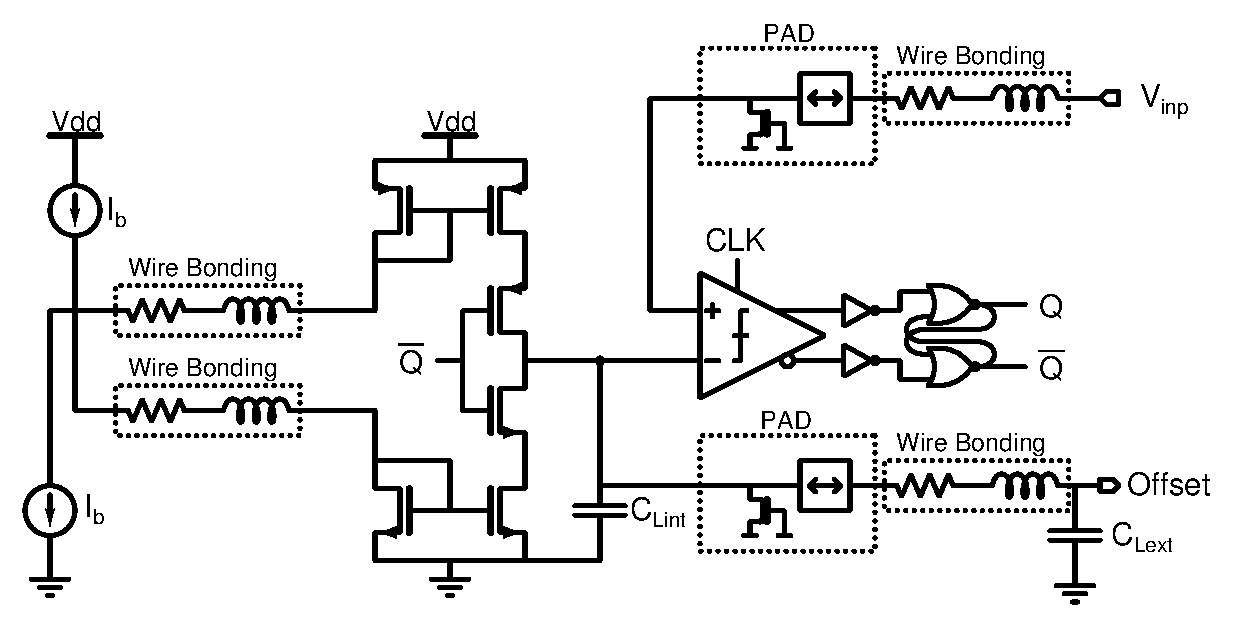
\includegraphics[width=\textwidth]{Chapter5/Figs/comp_test/feedback_offset_comp_principle.ps}
        \subcaption{schematic}
    \end{subfigure}
    \begin{subfigure}[b]{0.45\textwidth}
        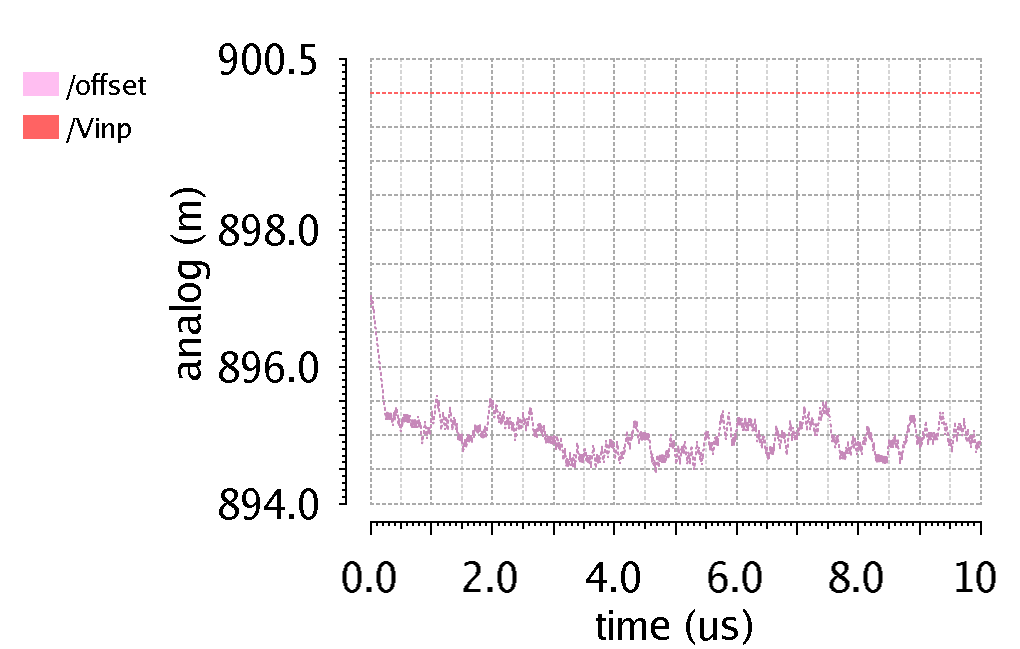
\includegraphics[width=\textwidth]{Chapter5/Figs/comp_test/fb_comp_offset_ref_res.png}
        \subcaption{transient voltage with initial condition}
    \end{subfigure}
    \caption{Test bench for the offset simulation which including pads and wire bonding with the noisy transient simulation for a comparator of reference}
    \label{fig:tb_fb_comp_offset}
\end{figure}

The \figurename~\ref{fig:tb_fb_comp_offset} a represents the schematic view of the test while the \figurename~\ref{fig:tb_fb_comp_offset} b depicts the signal seen over the simulation of a comparator with 5 mV offset and 1 mV rms noise. This test circuit has only one mode and is always on. By beginning with a reference voltage $V_{\rm inp}$ at 0 V, the offset voltage after few milliseconds will be at zero volt too. Then, the reference voltage steps up to the desired common-mode voltage. Therefore, the comparator will detect the difference between the two, and its memorized output will be 1. So, the charge pump circuit in the voltage generation bloc raises the OFB\_OFFSET voltage. With one transistor in saturation while the other is blocked, the current to load the capacitor is approximately the current defined by the $I_b$ over a full clock period of CLK. This pursues until the offset voltage is greater than the reference voltage. In this case, the current that charges the load capacitor is $–I_b$. Thence, the offset voltage starts to oscillate around the real input referred offset of the comparator.

\subsubsection{Bloc Description}
As represented in \figurename~\ref{fig:tb_fb_comp_offset} a, this circuit takes as an input two currents of reference which control the slewing of the feedback voltage OFFSET\@. In addition to that, a reference voltage called $V_{\rm inp}$ corresponds to the common-mode voltage at which we expect to test. The clock provided to the comparator control makes the comparator start a decision at its rising edge, while the comparator is reset when the clock is low. An SR-latch memorizes the output of the comparator under test before the reset. From the decision, the charge pump charges/or discharges an internal capacitor of 1.8 pF. The voltage generated OFFSET is used as the second input voltage of the comparator, and is connected to an output pad itself connected to an external capacitor to limit oscillations. Concerning the power supply, only one VDD and GND pins are needed. The voltage of the power supply is 1.8 V.

\subsubsection{source of perturbations}
In this circuit the external source of perturbations is the current source. Let us suppose the comparator operates in the same condition it will in the ADC\@, to wit $V_{DD}$ = 1.8 V and $F_{CLK}$ = 100 MHz. The comparator makes a decision every 10 ns. Due to the latency in the feedback loop, the variation of the offset voltage $\Delta$V is thus defined by the slewing: $\Delta V = \frac{I_b}{C_L F_{CLK}}$.

In a first approximation, the error committed by the circuit with a $C_L = C_{Lint} = 1.8 pF$, $I_b = 500 nA$ is 1.38 mV around the real value. In order to match the requirement of the 500 $\mu$V around the offset, the minimal capacitance should be at least 5.3 pF. This can be easily achieved by connecting an I/O pad directly to the probe of the measurement device and adding an external capacitor out of the chip of 2.2 pF: $C_L = C_{Lint} + C_{probe} + C_{Lext}$. This limiting the oscillations, but not annihilating them, we are interested in only the average value of the differential input.

Concerning phenomena from the comparator, the hysteresis will impact the desired voltage measurement. Indeed, having a different threshold voltage due to previous state of the comparator, the measured offset voltage will be oscillating between the two thresholds of the hysteresis. 
If the slope of the generated offset is very slow such that the variation peak-peak between two clock rising edge is less than the hysteresis, this phenomena is detected. If not, the average value still provides the information of the offset which is close to the average of the hysteresis threshold value.

Another phenomenon due to the comparator decision occurs: the kickback. The single-ended kickback is important since it will drop the voltage across the load capacitor, even if, the amplifier is always charging the capacitor. Therefore, the size of the capacitor is an important decision.
With a single-ended kickback of 500 mV over a 100 fF capacitor, by applying a rule of three, the kickback seen on a 1.8 pF plus an I/O pad will be 16 mV. The amplifier limiting the drop, this results in a 14.7 mV voltage drop on the offset voltage.


\subsubsection{Post-Layout Results}
Since neither the kickback nor the hysteresis is modelled in the comparator of reference, the information of whether the offset feedback circuit is able to cope with these phenomena is not known. Therefore, a post-layout comparator replaced the one of reference. Moreover, the schematic of the comparator and the extracted version of comparators have an adjusted offset around 5 mV to compare with the previous simulation results in \figurename~\ref{fig:tb_fb_comp_offset}. This allows us to compare only the impact of the phenomena not taken into account by the reference comparator. To wit, parasitic and the intrinsic hysteresis introduced by layout mismatch.

\begin{figure}[htp]
    \centering
    \begin{subfigure}[b]{0.48\textwidth}
        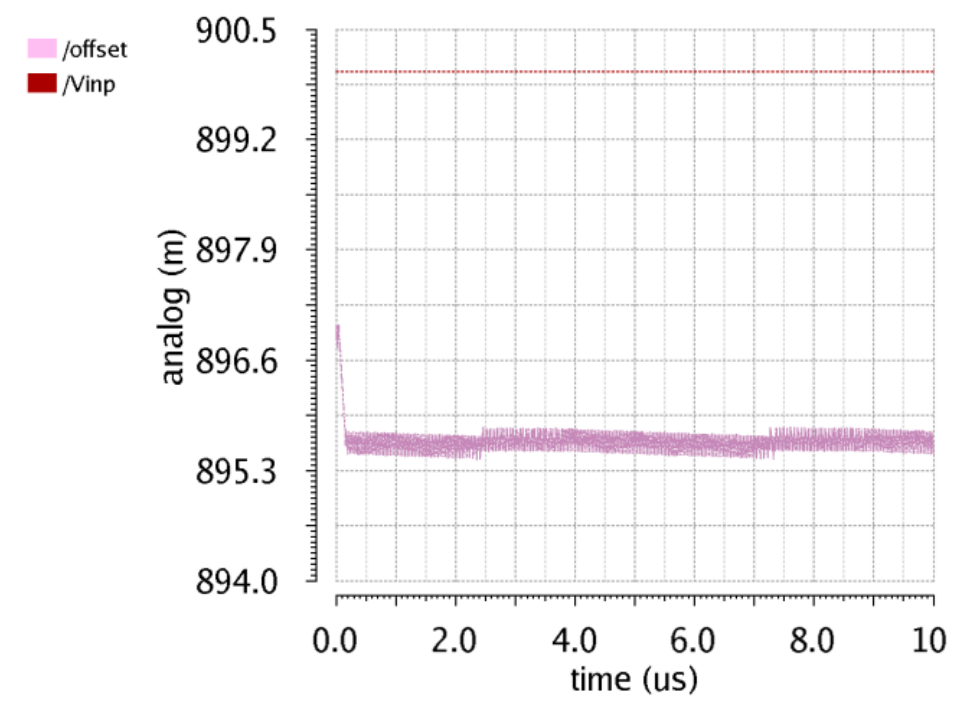
\includegraphics[width=\textwidth]{Chapter5/Figs/comp_test/comparator_offset_feedback_trans_real.png}
        \subcaption{Real comparator transient}
    \end{subfigure}
    \begin{subfigure}[b]{0.48\textwidth}
        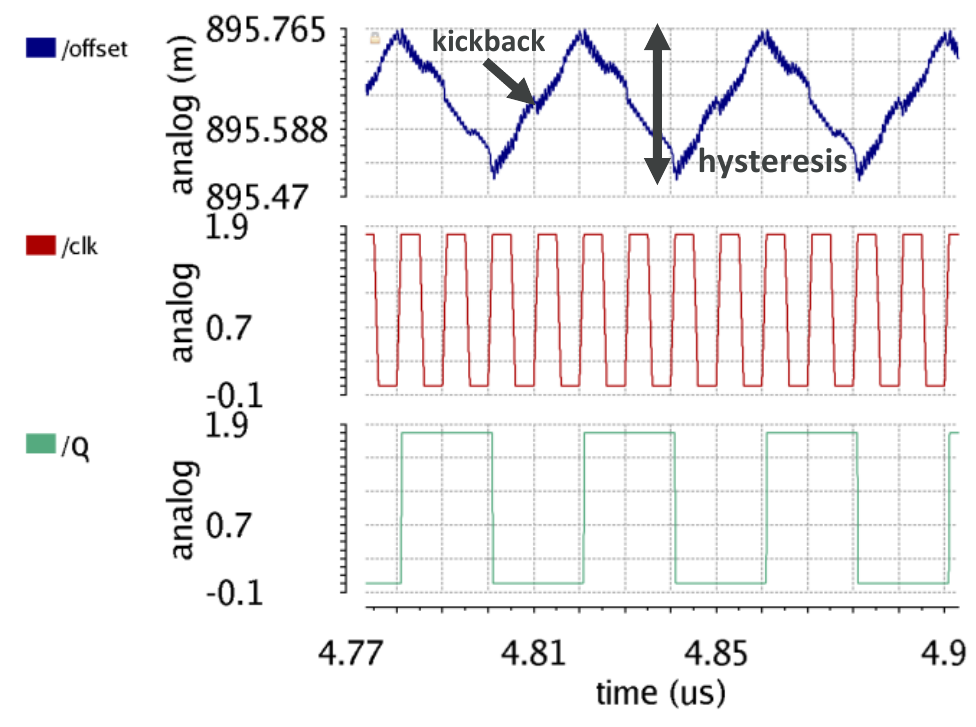
\includegraphics[width=\textwidth]{Chapter5/Figs/comp_test/comparator_offset_feedback_trans_real-zoom.png}
        \subcaption{Zoom on the kickback and hysteresis effect}
    \end{subfigure}
    \caption{Hysteresis and kickback effect on the offset feedback circuit at 27$\degree$C}
    \label{fig:comp_hyst}
\end{figure}

The transient offset voltage with the clock and the decision of the comparator alongside are depicted by the \figurename~\ref{fig:comp_hyst}. The results are for ambient temperature at 27$\degree$C. Since the current switching is low the voltage variation is fully delimited by the hysteresis of the comparator under test, to wit 325$\mu$V. With a large capacitive load split inside the chip and outside, the kickback is limited to few microvolts even for a clock at 100 MHz.

Running a Monte-Carlo analysis of comparators designed after parasitic extraction, the offset statistic of a slow double-tail comparator is compared to the traditional method of clocked comparator extraction used in Section~\ref{sec:latches_sim}. The Table~\ref{tbl:offset_fb_dtl_post_layout} presents the result under a 6$\sigma$ process and mismatch parameter variation at three different temperatures with 50 samples each.

\begin{table}[htp]
    \centering
    \caption{(Gaussian 6-$\sigma$) Monte-Carlo analysis results of the extracted offset for the double tail comparator with the current offset simulation}
    \label{tbl:offset_fb_dtl_post_layout}
    \begin{tabular}{cccccccc}
    \hline
    \multirow{2}{*}{Temperature/Offset} & \multirow{2}{*}{Min {[}mV{]}} & \multirow{2}{*}{Max {[}mV{]}} & \multicolumn{2}{c}{Mean {[}$\mu$V{]}} & \multicolumn{2}{c}{$\sigma_{offset}$ {[}mV{]}} & \multirow{2}{*}{$\Delta V$ {[}mV{]}} \\
                                        &                               &                               & Circuit           & Ref            & Circuit                 & Ref                  &                                   \\ \hline
    -50$\degree$C                          & -1.89                         & 2.72                          & 269               & 290            & 1.27                    & 1.73                 & 1.16                              \\
    27$\degree$C                           & -2.14                         & 3.47                          & 570               & 620            & 1.39                    & 1.84                 & 2.33                              \\
    175$\degree$C                          & 3.33                          & 6.6                           & 1000              & 1410           & 2.29                    & 2.44                 & 4.64                              \\ \hline
    \end{tabular}
\end{table}

The circuit is relevant for low-temperature measurement with an accuracy of 50 \(\mu\)V. Owing to thermal noise and hysteresis at high temperature the accuracy of the circuit decrease to 400 \(\mu\)V on the mean. A possibility to enhance results is by the averaging of the offset voltage lasting longer in time than 1\(\mu\)s (1000 comparator decision) to mitigate the transient noise in measurement with twice more samples. Unfortunately a lack of time available for the tests did not permit us to collected experimental data. This is scheduled to happen later on.

\subsection{Test Pattern C: Conventional Offset, Hysteresis, and Noise measurement}
At our best knowledge, Test Pattern B has only been used in simulation~\cite{1594475}. In order to compare with the most common methodology to measure the offset, this conventional method has also been implemented in DOE\_COMP. In addition to offset measurement, this circuit allows the extraction of the comparator's hysteresis and its intrinsic noise.

From the design of comparators, the target offset is as close as possible from zero with a standard deviation of 3 mV. Based on that, the accuracy needed is less 500 $\mu$V\footnotemark for a maximum error of 5\% on the standard deviation. \footnotetext{see Appendix~\ref{app:acc-offset} for the details of the calculation}

\subsubsection{Principle}
As represented in \figurename~\ref{fig:conv_offset}, this solution consists in counting the number of ones and zeros generated by comparators under test, for each differential input voltage distributed evenly around the common mode voltage. Therefore, each differential input voltage is associated with a ratio of ones counted over the maximum possible values in the test time. This corresponds to averaging the comparator output for each differential input voltage. By sweeping the input voltages of the comparator, we get an S-shaped probability distribution.

\begin{figure}[htp]
    \centering
    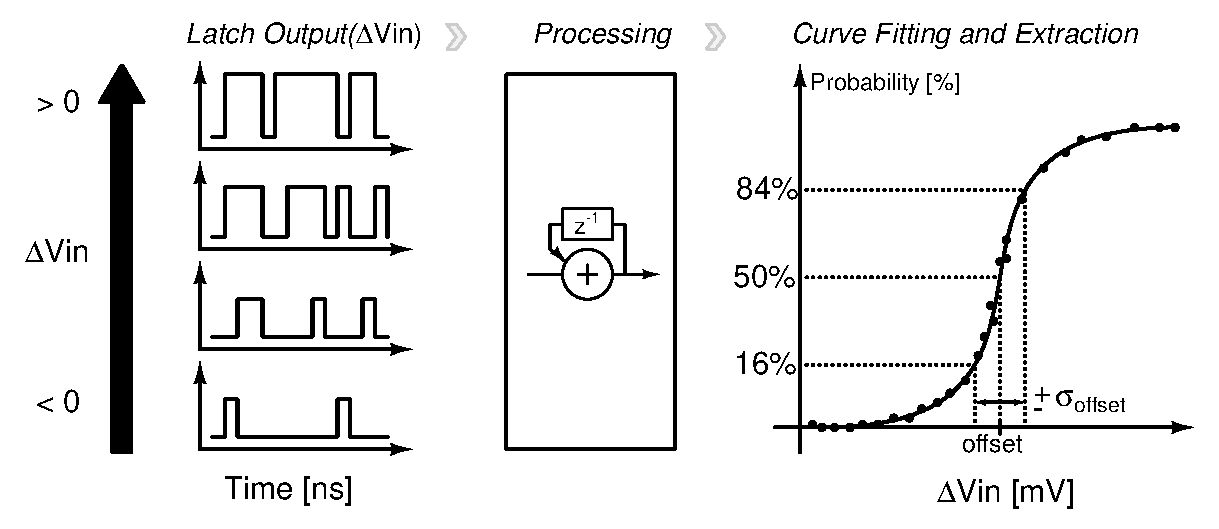
\includegraphics[width=.8\textwidth]{Chapter5/Figs/comp_test/offset_conv_principle.ps}
    \caption{Typical principle to measure the offset of comparators based on the variation of the differential input voltage}
    \label{fig:conv_offset}
\end{figure}

Without offset, the inflexion point of the curve plotted should be equal to the common-mode voltage: $\Delta V_{in} = 0$. And a small shift corresponds to the offset. This solution is the most common for measurement of the offset~\cite{4395036,6482245,6644886}.

The advantage of such circuit is the resilience to cope with the thermal noise. At a given clock frequency, the smallest differential input voltage is set by the one who test. But for a tiny differential input, the noise will trigger the comparator under test, and its outputs are either 1 or 0. An assumed white thermal noise will produce an evenly repartition of 1 and 0, thence only few bits over thousands shift the probability to output one. This makes a smoother transition from quasi-zero to quasi-one probability. This results only in a change of the standard deviation.

From the density function to output a one, we fit the data with the cumulative distribution function of a Normal distribution. The fitting will average the error due the white Gaussian noise while it estimates the average and the standard deviation of the offset. The average, equal to the inflexion point of the curve, corresponds to the offset, and ideally occurs for a probability of 50\%. And the standard deviation of the offset corresponds to the noise contribution. There is no preferred algorithm for the fitting, so we used Levenberg-Marquardt to minimize the error committed on the fitting.

Moreover, applying this procedure over several comparators allows us to calculate the average of the offset and its standard deviation with respect to process and mismatch. This time, the probability curve should be the average of each comparator probability curve. The average offset is thus defined by the differential input voltage which corresponds to the 50\% of the new probability. And the standard deviation is extracted from the 68.27\% probability range around the new inflexion point.

\subsubsection{Curve Fitting Limitation}
For a comparator without hysteresis, the probability to output a one for each $\Delta V_{\rm in}$ is similar to what is represented in the \figurename~\ref{fig:conv_offset}. With an hysteresis, \figurename~\ref{fig:conv_offset_hyst}, the transition of probability will be slightly sharper. In order, the highlight the presence of hysteresis, the differential input voltage should be progressively changing from negative values to positive values then from positive values to negative values. The presence of hysteresis will demonstrate two S-shapes shifted from one to the other. The $\Delta$V shift of the offset value corresponds to the hysteresis while $\Delta V_{\rm in1}$ and $\Delta V_{\rm in2}$ represent the offset voltage. To correctly estimates, the data should be split to have one fitting when the differential input is increasing, and one when the differential input is decreasing.

\begin{figure}[htp]
    \centering
    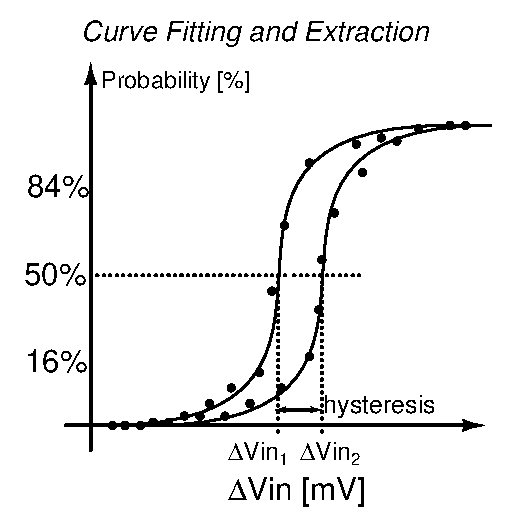
\includegraphics[width=.3\textwidth]{Chapter5/Figs/comp_test/offset_conv_principle_hyst.ps}
    \caption{Measurement of the hysteresis by sweeping back and forth the input voltages of comparators}
    \label{fig:conv_offset_hyst}
\end{figure}

About the choice of the input voltage, the input referred offset is in the $\pm$ 10 mV range. Therefore, the $\Delta V$ in shall be from -20 mV to +20 mV to ensure some margin. And to respect the requirement on the accuracy, a step between two consecutive differential input voltages should be less than 500 $\mu$V.

From a fitting point of view, the less noise there is, the fewer the number of points is in the transition. In consequence, the step between two consecutive differential input voltages might not be sufficient to estimate the noise accurately. By simulation, the standard deviation of the noise is 480 $\mu$V rms such that a 3$\sigma$ transition is expected to have 9 points. 

\subsubsection{Bloc Description}
The analogue part of the conventional test circuit is represented in the \figurename~\ref{fig:test-chip-comp-patterns-conv}. This part is made of 16 comparators with their inverters and SR-latch next to them. Among those comparators, there are 8 Strong Arm and 8 Double Tail comparators taking their decision at the same time. Inverters decouple the comparator output from the SR-latch who memorized the output. The inverter's outputs are considered to be analog, while the output of the SR-latch is assumed to be digital.

\begin{figure}[htp]
    \centering
    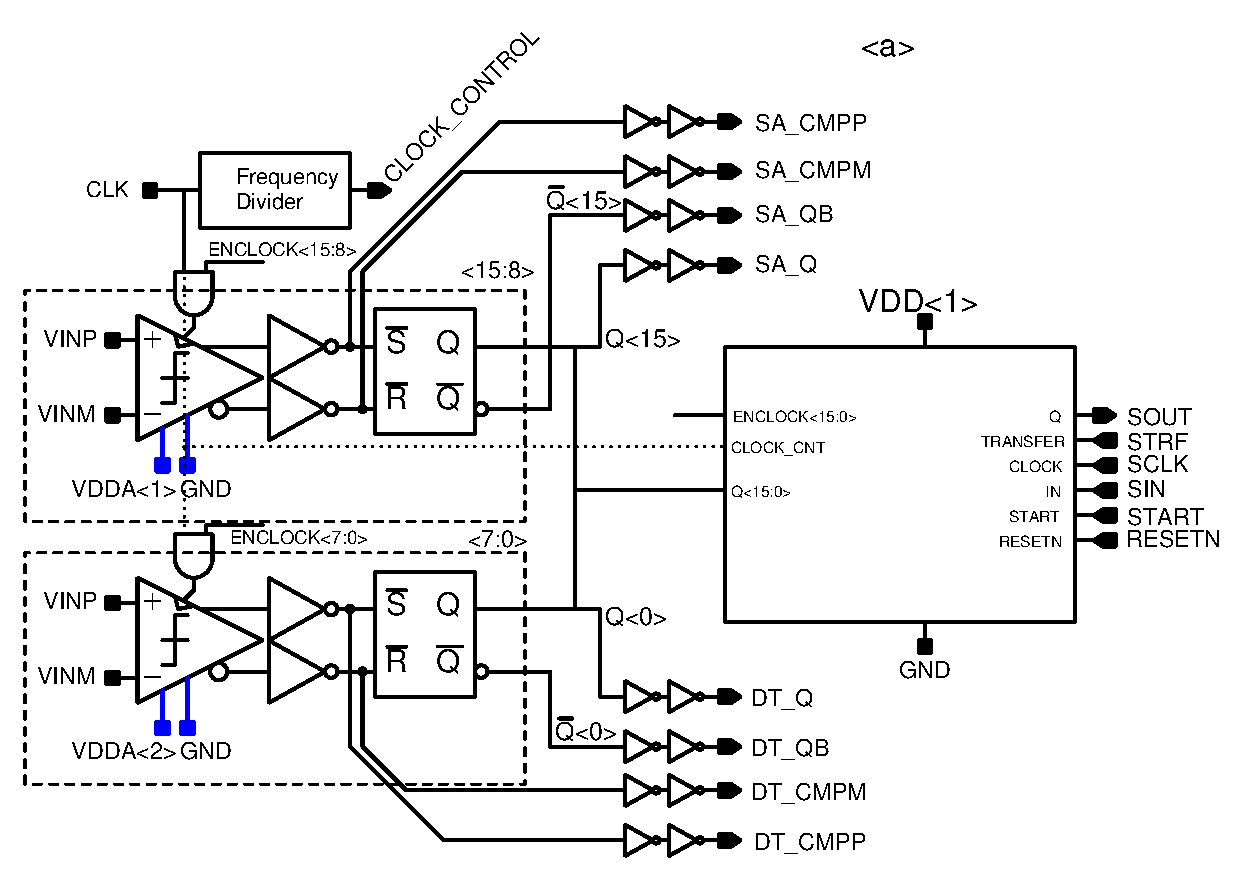
\includegraphics[width=0.75\textwidth]{Chapter5/Figs/comp_test/test_offset_conv_bloc.ps}
    \caption{Conventional offset measurement circuit to measure the offset, the hysteresis and the noise of 16 comparators (8 Strong-ARM and 8 Double-Tail)}
    \label{fig:test-chip-comp-patterns-conv}
\end{figure}

\begin{figure}[htp]
    \centering
    \begin{subfigure}[b]{0.48\textwidth}
        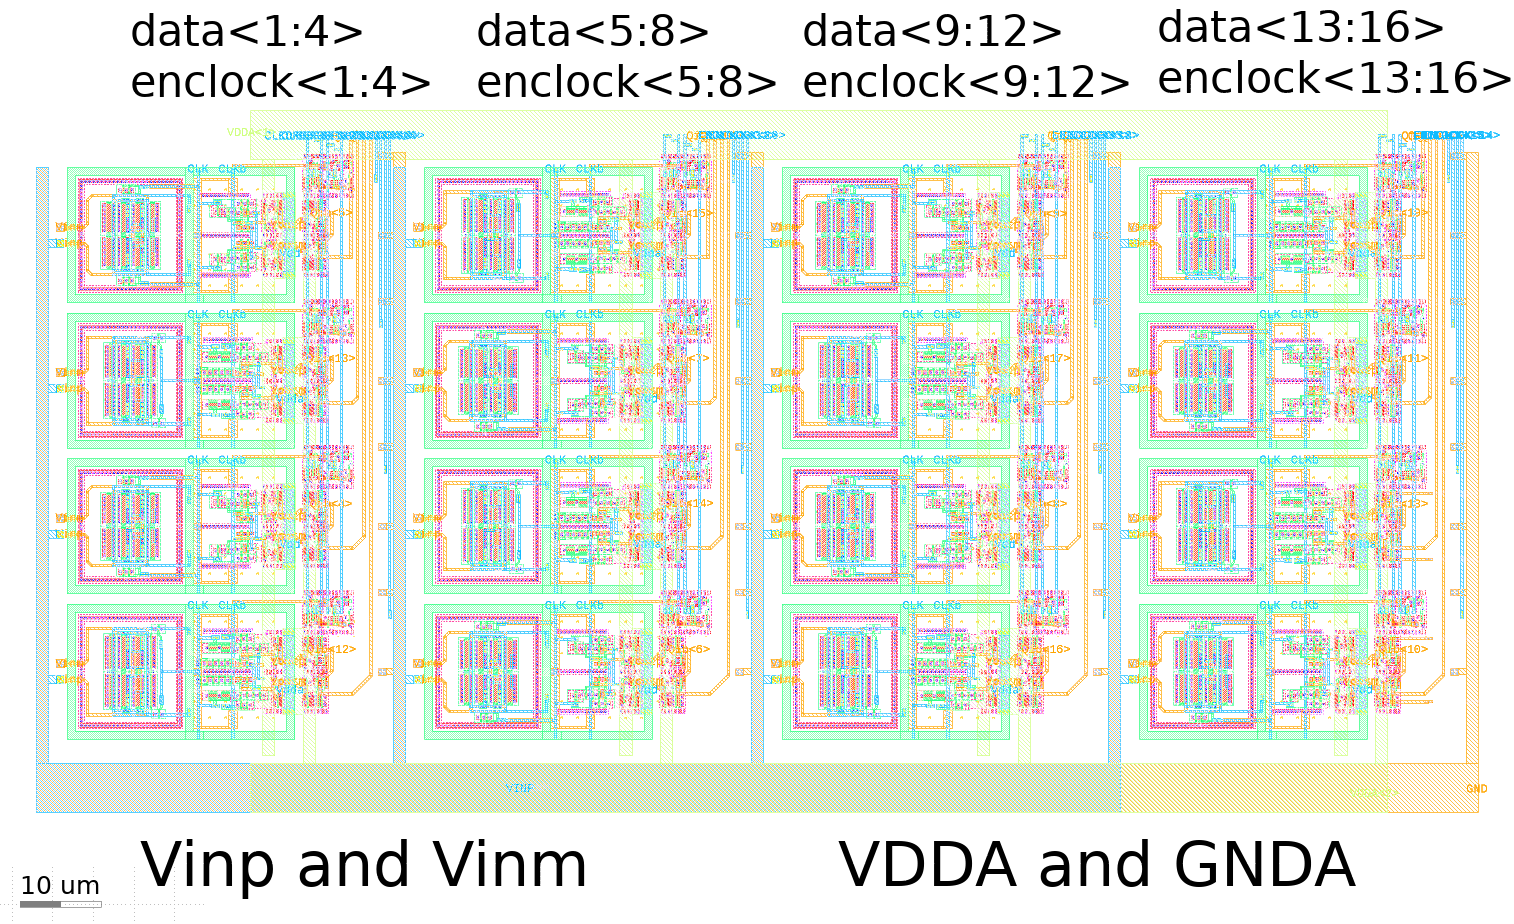
\includegraphics[width=\textwidth]{Chapter5/Figs/comp_test/comparator_analog_offset_layout.png}
        \subcaption{Analogue Placement}
    \end{subfigure}
    \begin{subfigure}[b]{0.48\textwidth}
        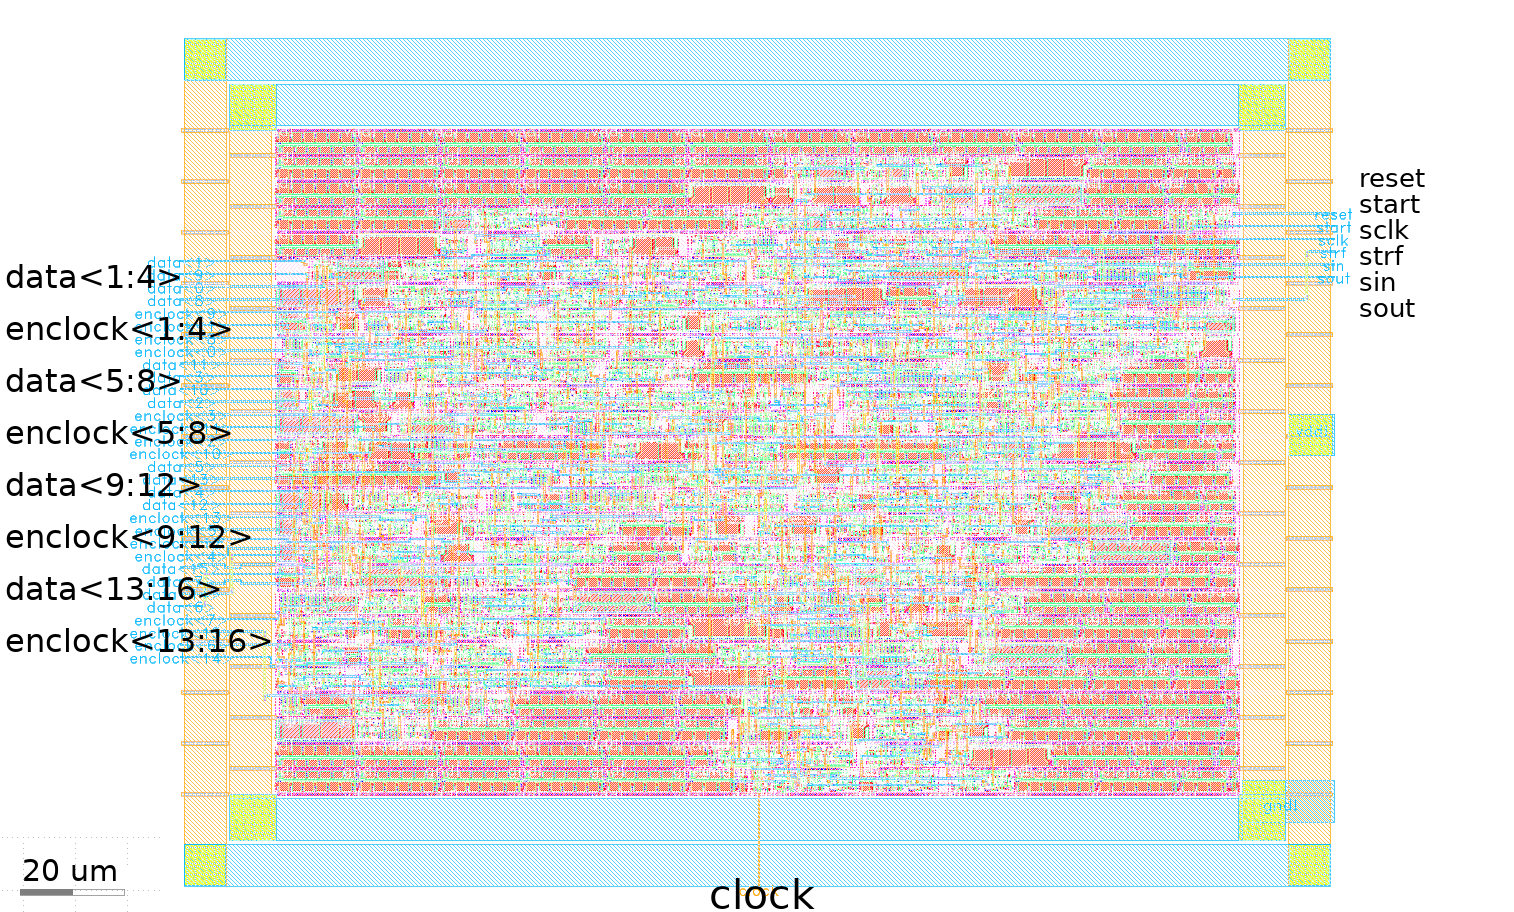
\includegraphics[width=\textwidth]{Chapter5/Figs/comp_test/comparator_digital_offset_layout.png}
        \subcaption{Digital Bloc and signal selection}
    \end{subfigure}
    \caption{Comparator test chip overview with 20 comparators to test the delay, the offset of the both comparator topologies. One extra delay test circuit is for diagnostic purpose}
    \label{fig:comp_offset_layout}
\end{figure}

The interleaved repartition into even index for strong arm and odd index for double tail, in \figurename~\ref{fig:comp_offset_layout} a, prevents the performance degradation of one comparator in favor of the other by having the same voltage drops for both topologies.

As represented in \figurename~\ref{fig:comp_offset_layout} b, the outputs of the 16 comparators enter the digital bloc which selects which one is counted. To configure which comparator is selected, 4 bits are transferred through SIN with respect to its clock SCLK\@. Then 16 bits are transferred in order to select which comparators are taking decisions which control the ENCLOCK signals. The last bit is validated by a STRF pulse which replies by sending the output of the internal counter of 1s.

\begin{figure}[htp]
    \centering
    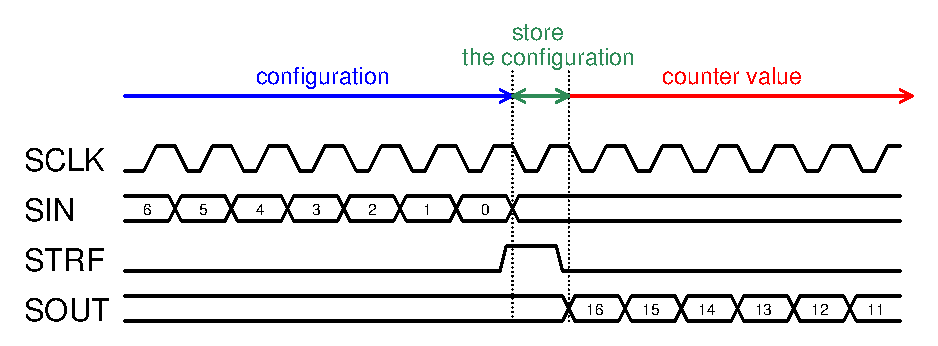
\includegraphics[width=0.8\textwidth]{Chapter5/Figs/comp_test/configuration-patternc.ps}
    \label{fig:test-comp-pattern-c-config}
    \caption{Configuration signal to validate the configuration and the counter value reading}
\end{figure}

\subsubsection{Simulation Results}
In order to verify that the probability model chosen is correct, the input file of the post-processing script is obtained by simulation of the test bench with a comparator of Reference. While one input voltage is set to the common mode voltage, the other is a triangle waveform from $V_{cm}-20 mV$ to $V_{cm}+20 mV$ by step of 0.5 mV. The expected offset and the expected standard deviation of the offset are respectively 5 mV and 1 mV with an hysteresis of 1 mV. The simulation at 27$\degree$C, gives the results presented in the \figurename~\ref{fig:offset_conv_verif}.

\begin{figure}[htp]
    \centering
    \begin{subfigure}[b]{0.32\textwidth}
        \adjincludegraphics[trim={{0.01\width} 0 {0.657\width} 0},clip,width=\textwidth]{Chapter5/Figs/comp_test/offset_conv_comp_ref_res.png}
        \subcaption{Offset}
    \end{subfigure}
    \begin{subfigure}[b]{0.32\textwidth}
        \adjincludegraphics[trim={{0.345\width} 0 {0.33\width} 0},clip,width=\textwidth]{Chapter5/Figs/comp_test/offset_conv_comp_ref_res.png}
        \subcaption{Standard deviation}
    \end{subfigure}
    \begin{subfigure}[b]{0.32\textwidth}
        \adjincludegraphics[trim={{0.675\width} 0 0 0},clip,width=\textwidth]{Chapter5/Figs/comp_test/offset_conv_comp_ref_res.png}
        \subcaption{Hysteresis}
    \end{subfigure}
    \caption{Extracted offset and standard variation of the offset for the comparator of reference at all positions}
    \label{fig:offset_conv_verif}
\end{figure}

In simulation, the average offset is as represented in \figurename~\ref{fig:offset_conv_verif} a. The estimation for each comparator gives 5 mV as expected. And since there is only the noise which impact the slope of the rising probability of one, the standard variation should be equal too. In the \figurename~\ref{fig:offset_conv_verif} b, the estimation of the standard deviation is around this value. Therefore, the methodology applied extracts correctly the information of the offset for the comparator of reference.

Then, the comparators are changed for a Double-Tail comparator as done in other tests. First, the impact of the temperature is studied for 5 temperatures linearly distributed in the -50$\degree$C -- +175$\degree$C range. Nothing is changed between the simulation of the reference comparator and this test.
The results for the temperature variation are presented in the \figurename~\ref{fig:offset_conv_dtl} which represents the offset variation, its standard deviation, and the hysteresis with respect to the temperature for the slowest version of the Double Tail. A Gaussian variation of parameters due to mismatch around this corner is performed.

\begin{figure}[htp]
    \centering
    \begin{subfigure}[b]{0.32\textwidth}
        \adjincludegraphics[trim={{0.01\width} 0 {0.657\width} 0},clip,width=\textwidth]{Chapter5/Figs/comp_test/offset_conv_comp_dtl_res.png}
        \subcaption{Offset}
    \end{subfigure}
    \begin{subfigure}[b]{0.32\textwidth}
        \adjincludegraphics[trim={{0.345\width} 0 {0.33\width} 0},clip,width=\textwidth]{Chapter5/Figs/comp_test/offset_conv_comp_dtl_res.png}
        \subcaption{Standard deviation}
    \end{subfigure}
    \begin{subfigure}[b]{0.32\textwidth}
        \adjincludegraphics[trim={{0.675\width} 0 0 0},clip,width=\textwidth]{Chapter5/Figs/comp_test/offset_conv_comp_dtl_res.png}
        \subcaption{Hysteresis}
    \end{subfigure}
    \caption{Extracted offset and standard variation of the offset for the slowest double tail}
    \label{fig:offset_conv_dtl}
\end{figure}

The proposed circuit is able to operate even for a comparator which is really slow and over temperature. The variation with respect to the temperature behaves as expected. The standard deviation of the offset corresponds to the results found in section~\ref{sec:latches_sim}, while the mean of the offset is centered on 0.

For practical reasons related in Appendix~\ref{app:Packaging}, most of samples taped out does not gives relevant results. While most of them does not have a configuration link properly connected, those whose configuration operate as expected has been partially tested. 
